\section{Controles} % 5.3 Controls

\change[inline]{Map out the game procedures and controls. Use visualizations
like control tables and flowcharts, along with descriptions.}

\subsection{Acciones}

\change[inline]{Las acciones son aquellas cosas que puede hacer el jugador
dentro del juego. Se agruparán según a qué modo pertenecen.}

La acción que podrá realizar el jugador en la mayoría de modos es:
\begin{itemize}
    \item Acceder a la configuración general
\end{itemize}
El único modo en el que no puede realizar esta acción es el modo partida.

\subsubsection{Modo menú principal}
\begin{itemize}
    \item Acceder al menú de selección de perfiles
    \item Salir del juego
\end{itemize}

\subsubsection{Modo selección de perfil}
\begin{itemize}
    \item Borrar perfil
    \item Crear perfil
    \item Entrar al perfil
    \item Volver al menú principal
\end{itemize}

\subsubsection{Modo perfil}
\begin{itemize}
    \item Crear nueva partida
    \item Cambiar configuracion de perfil
    \item Volver al menú de selección de perfil
\end{itemize}

\subsubsection{Modo configuración de partida}
\begin{itemize}
    \item Configurar datos de la partida
    \item Entrar al menú de selección de personaje (Crear partida)
    \item Volver al perfil
\end{itemize}

\subsubsection{Modo selección de personaje}
\begin{itemize}
    \item Cambiar de personaje
    \item Seleccionar personaje (Necesario para empezar partida)
    \item Volver al menú de configuración de partida
\end{itemize}

\subsubsection{Modo partida}
\change[inline]{No se puede acceder al menú de configuración general desde aquí directamente}

\begin{itemize}
    \item Moverse
    \item Atacar
    \item Usar habilidad
    \item Usar objeto
    \item Recolectar objeto
    \item Descartar objeto
    \item Interactuar con NPC
    \item Recolectar monedas
    \item Comprar objeto
    \item Pausar
    \item Avanzar de nivel
\end{itemize}

\subsubsection{Modo pausa}
\begin{itemize}
    \item Abandonar partida
    \item Volver a la partida
\end{itemize}

\subsubsection{Modo victoria}
\begin{itemize}
    \item Salir de la partida
\end{itemize}

\subsubsection{Modo derrota}
\begin{itemize}
    \item Salir de la partida
\end{itemize}

\subsubsection{Modo configuración}
\begin{itemize}
    \item Cambiar el volumen del audio
\end{itemize}

\subsection{Interacciones}
% Lo que hacen los NPCs y monstruos

% Las plataformas también son entidades y por tanto:
% Colisionar
% Moverse
% Desaparecer
% Rotar
% Efecto especial?

\subsection{Condiciones de victoria/puntuación} % 5.3.3 Scoring/winning conditions

\change[inline]{Describe the scoring system and win conditions. These might be
different for single player versus multiplayer or if you have several modes of
competition.}
\begin{itemize}
    \item Llegar a la cima de la torre primero (condición de victoria)
    \item Derrotar enemigos
    \item Derrotar jefes
    \item Impedir el progreso de otro jugador
\end{itemize}

\subsection{Reglas} %     5.3.2 Rules

\change[inline]{If you have created a prototype, describing the rules of your
game will be much easier. You will need to define all the game objects,
concepts, their behaviors, and how they relate to one another in this section}

\subsection{Interfaces} %     5.3.1 Interfaces

\change[inline]{Create wireframes, as described on page 439, for every interface
the artists will need to create. Each wireframe should include a description of
how each interface feature functions. Make sure you detail out the various
states for each interface.}

\urgent{NO OLVIDES AÑADIR LA DESCRIPCIÓN DE CADA ELEMENTO DE CADA INTERFAZ}

\subsubsection{Modo menú principal}
\begin{figure}[H]
    \centering
    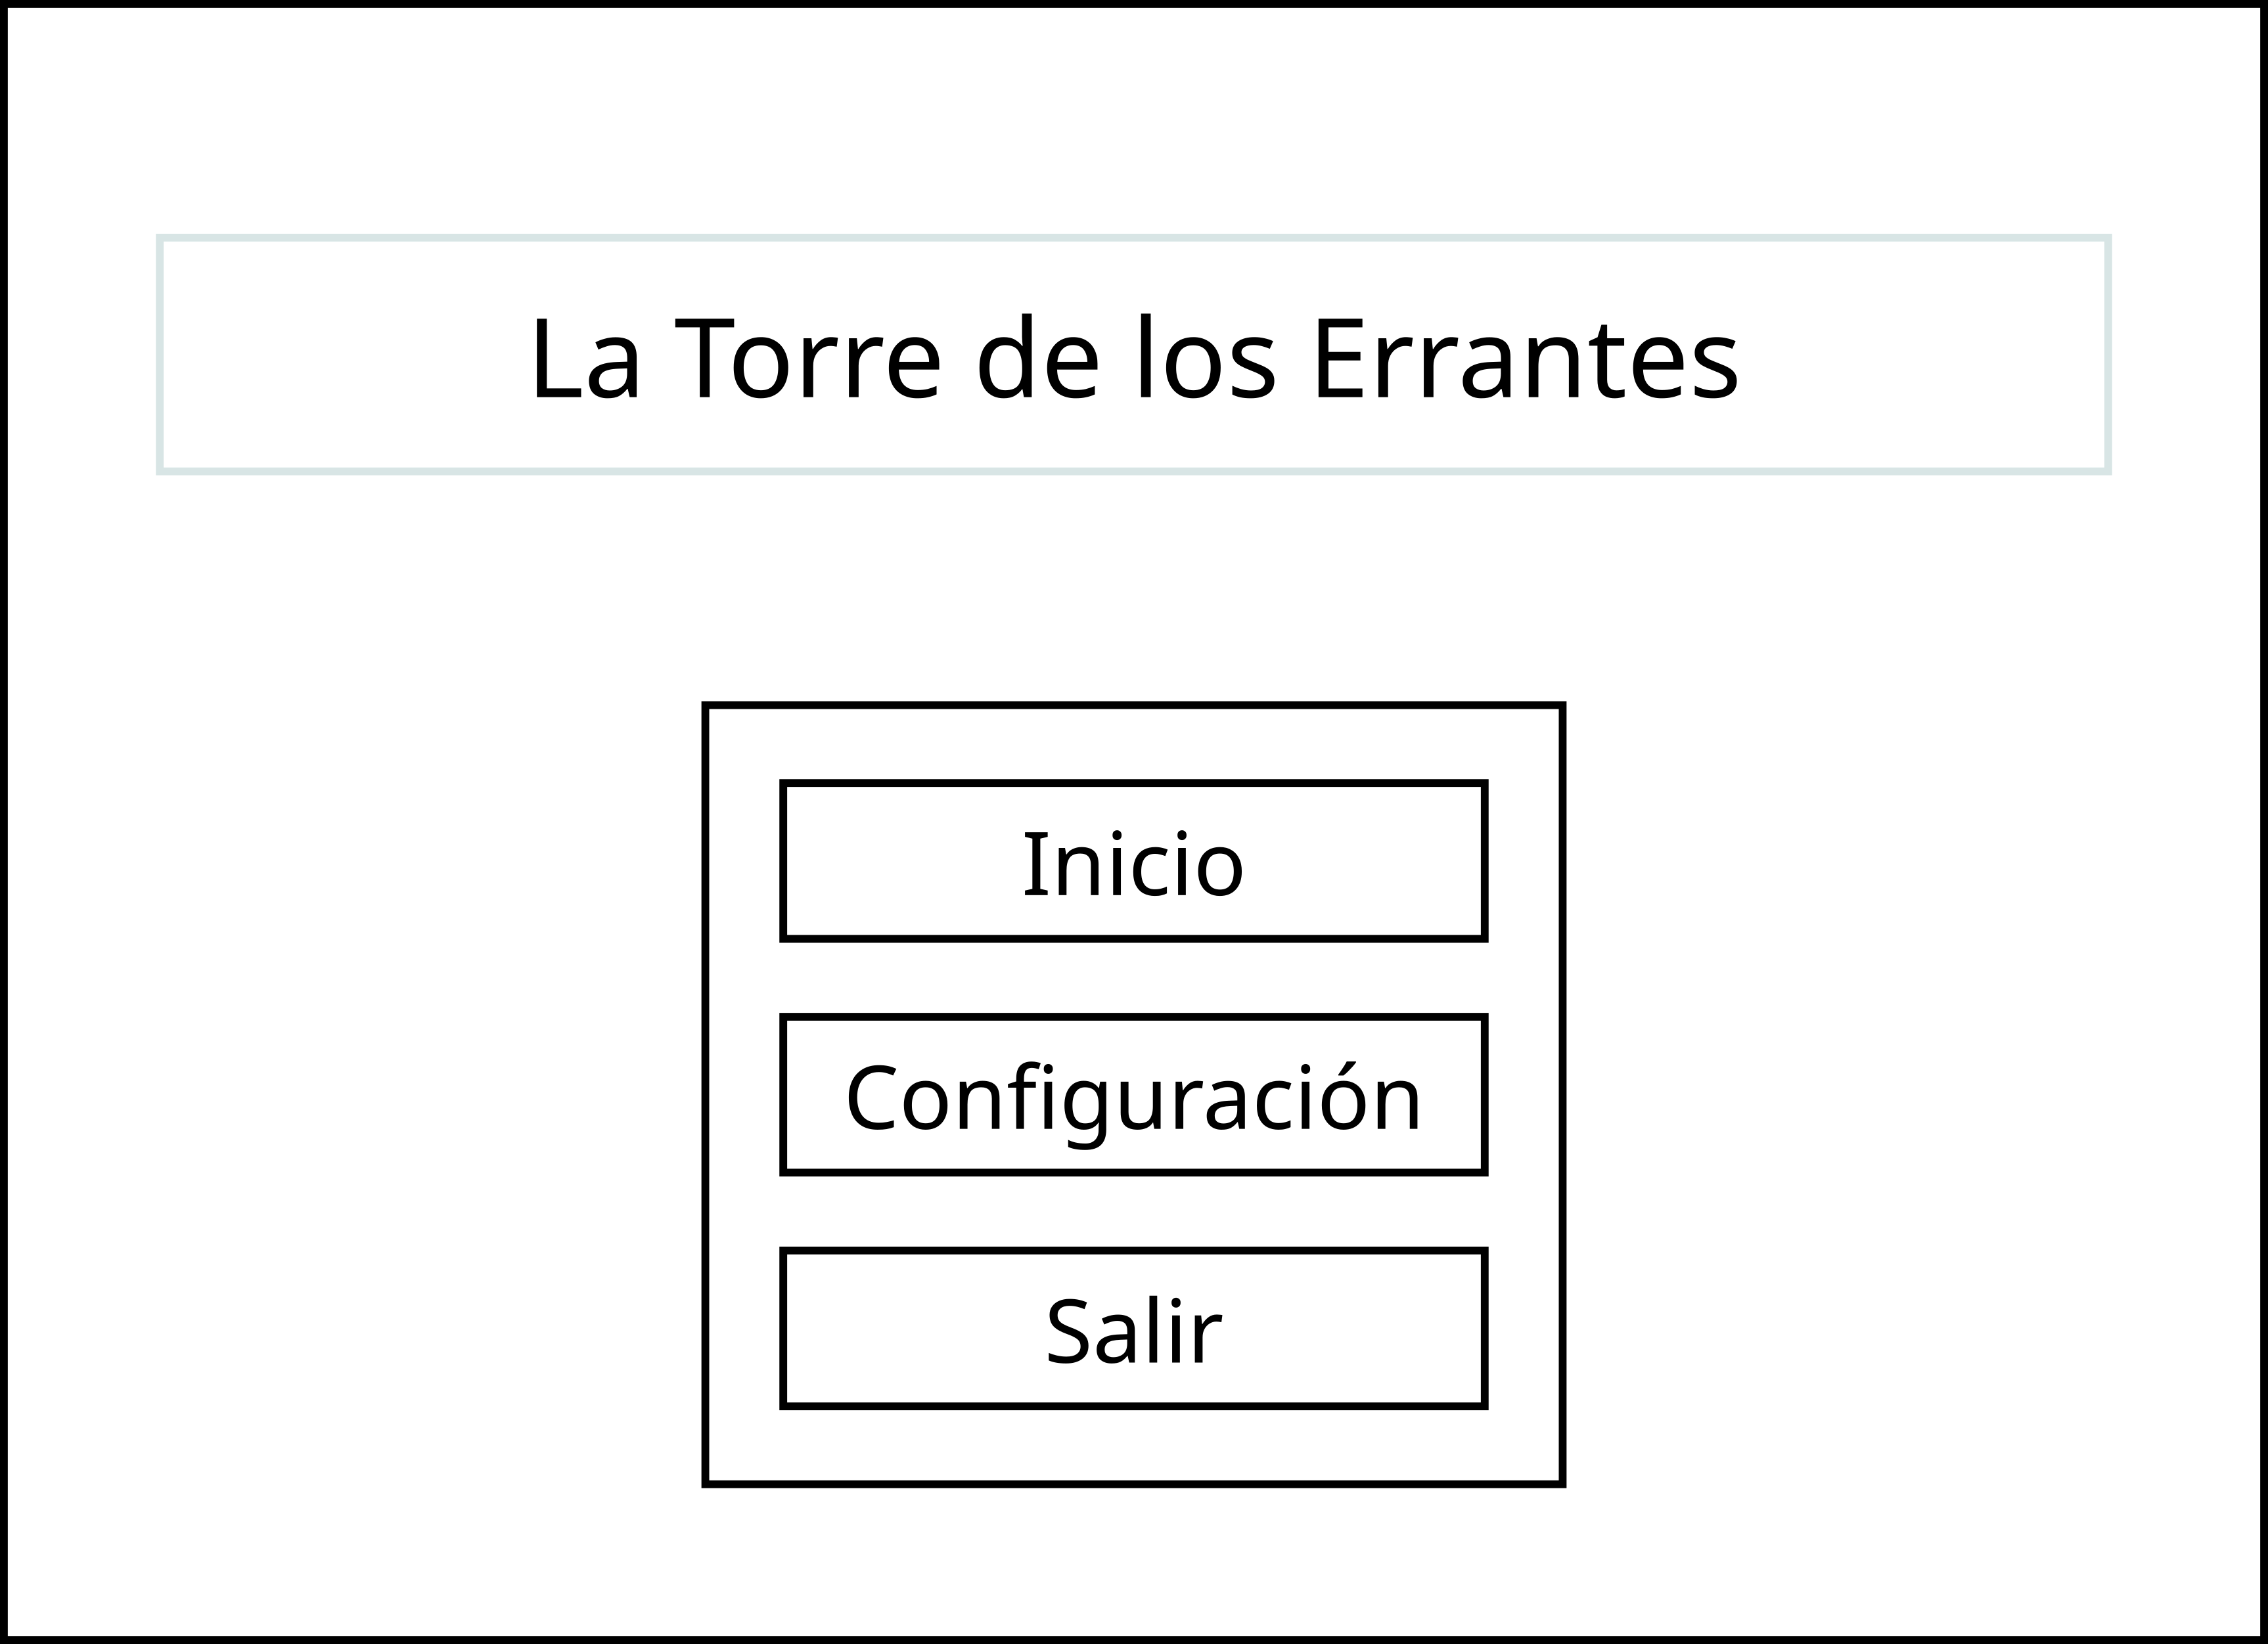
\includegraphics[width=0.6\textwidth]{5-Cuerpo/Chapter5/I1.png} %
    \caption{Interfaz del menú principal}
    \label{fig:Interface_Menu_Principal}
\end{figure}
\begin{enumerate}\setcounter{enumi}{-1}
    \item 0
    \item 1
    \item 2
    \item 3
\end{enumerate}

\subsubsection{Modo selección de perfil}
\begin{figure}[H]
    \centering
    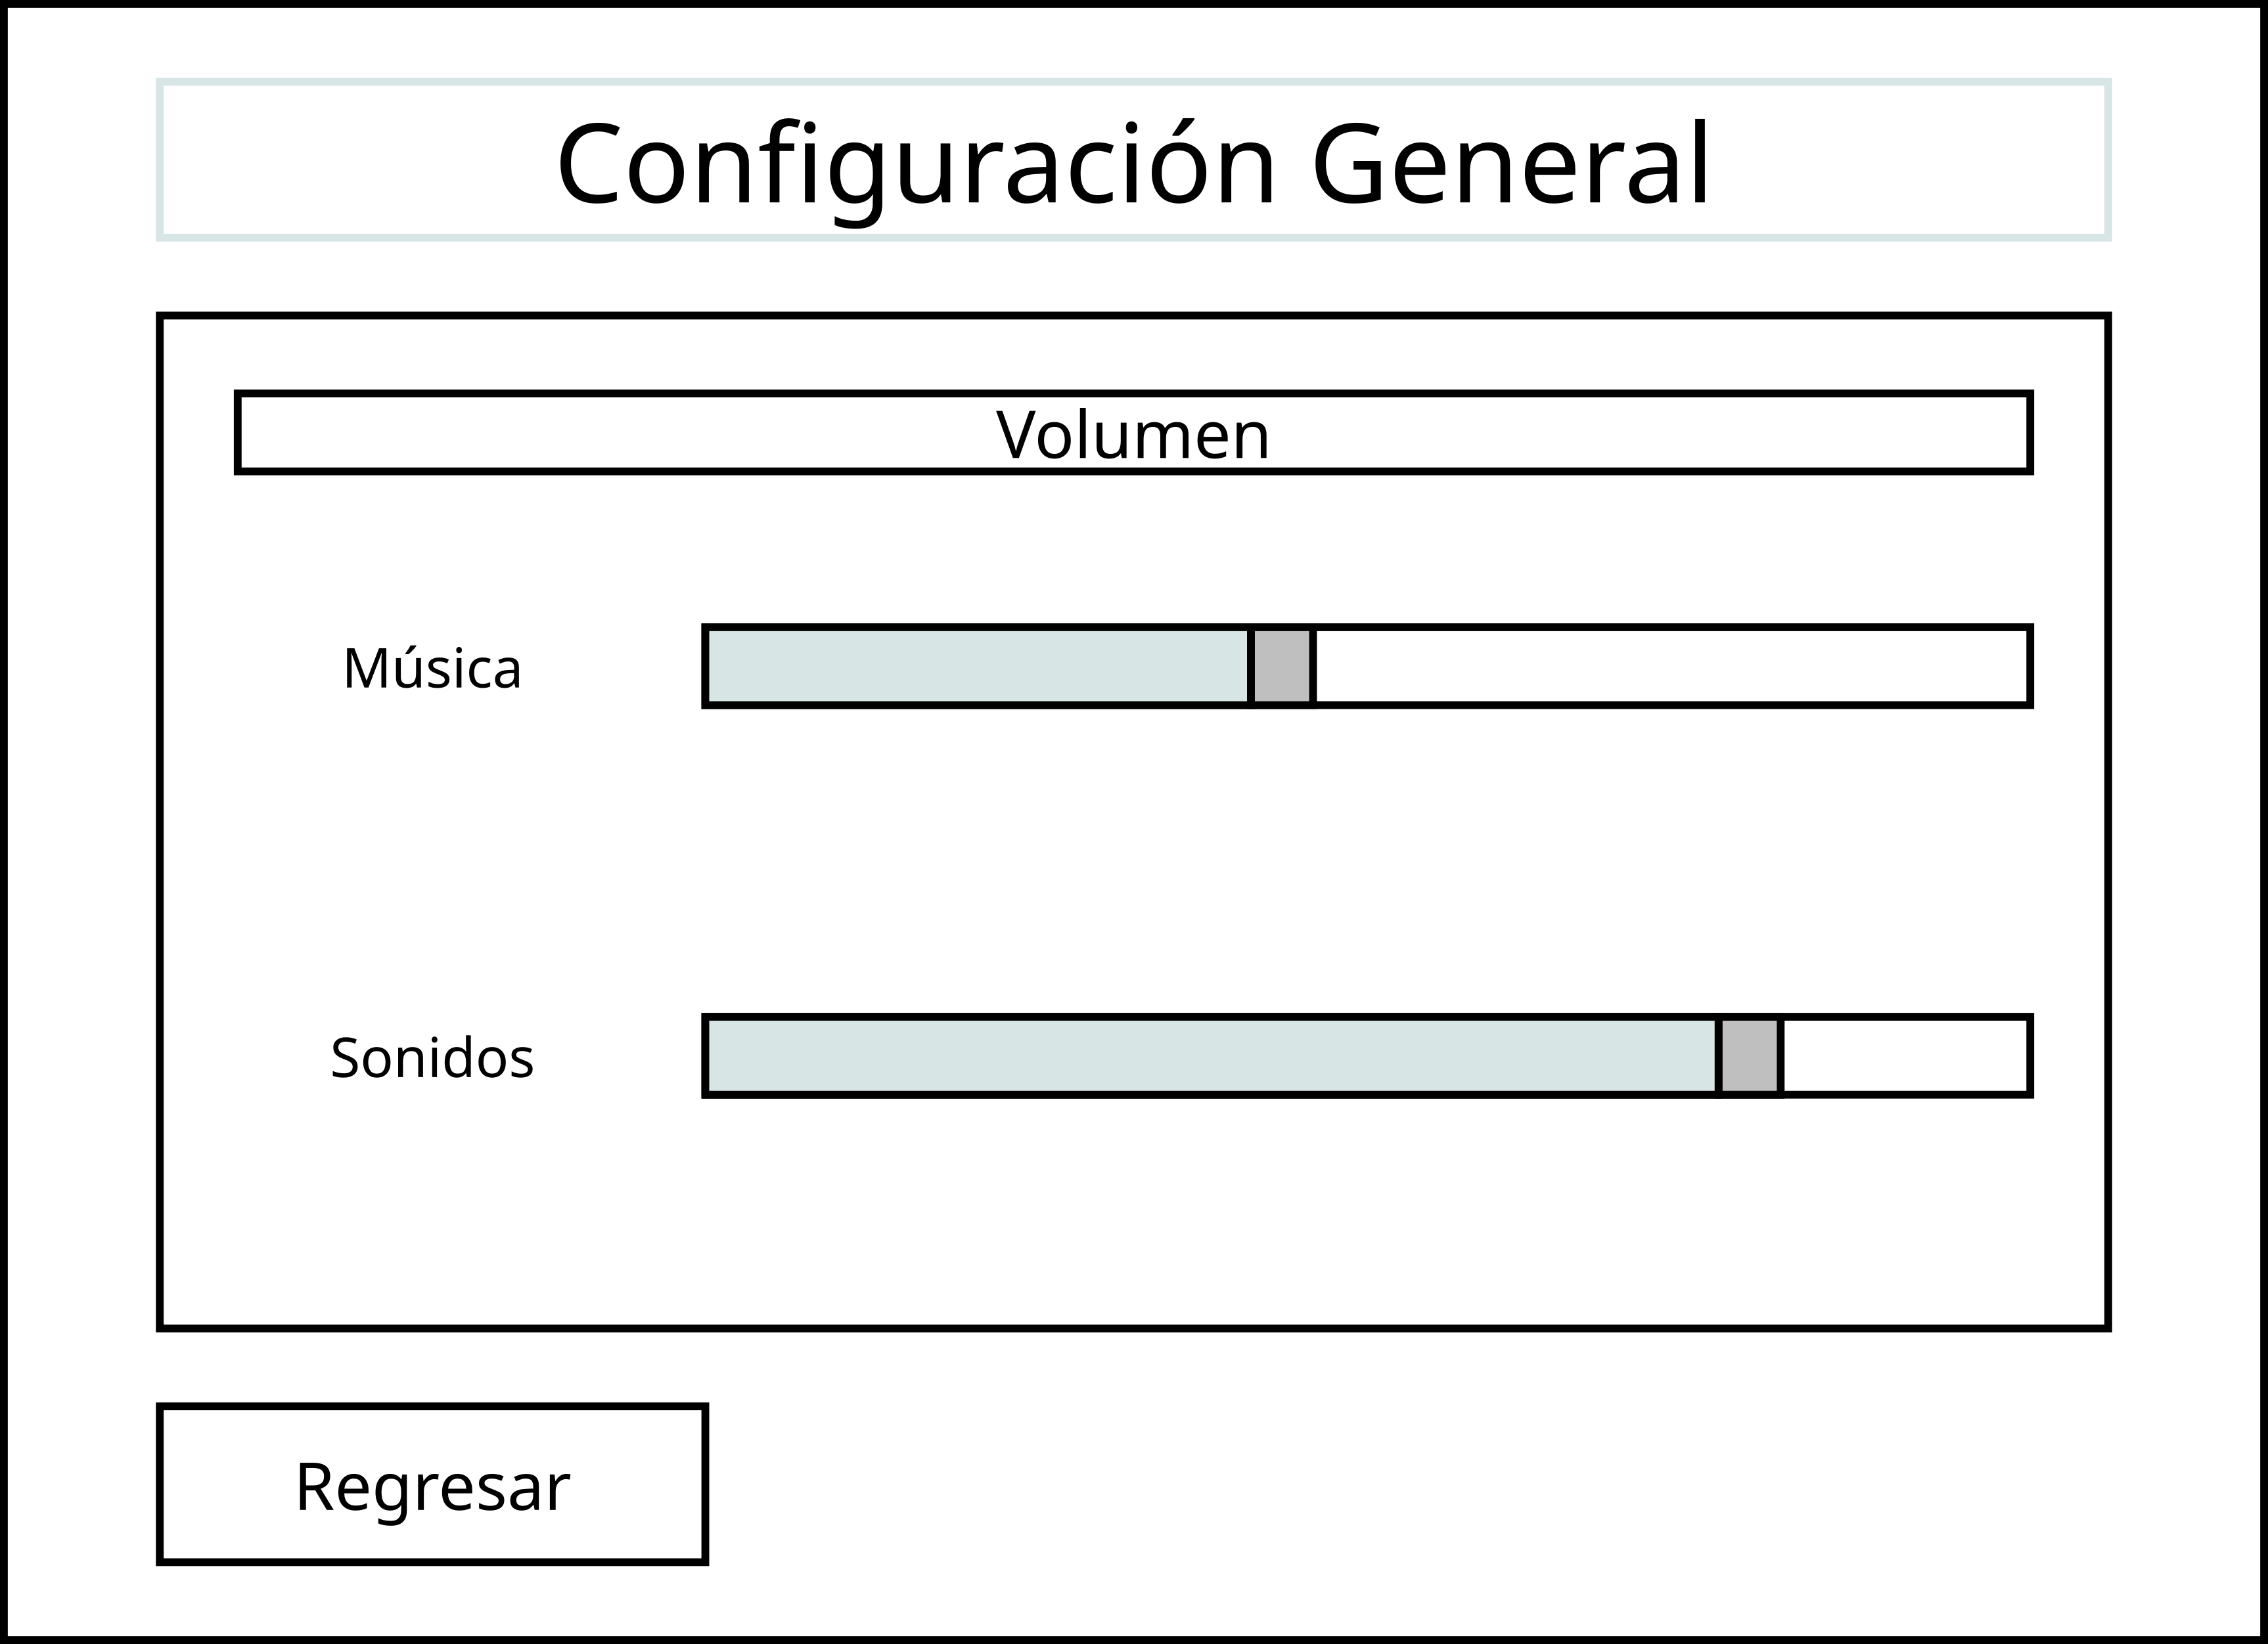
\includegraphics[width=0.6\textwidth]{5-Cuerpo/Chapter5/I2.png} %
    \caption{Interfaz del menú de selección de perfiles}
    \label{fig:Interface_Seleccion_Perfil}
\end{figure}
\begin{enumerate}\setcounter{enumi}{3}
    \item 4
    \item 5
    \item 6
    \item 7
    \item 8
    \item 9
    \item 10
\end{enumerate}

\subsubsection{Modo perfil}
\begin{figure}[H]
    \centering
    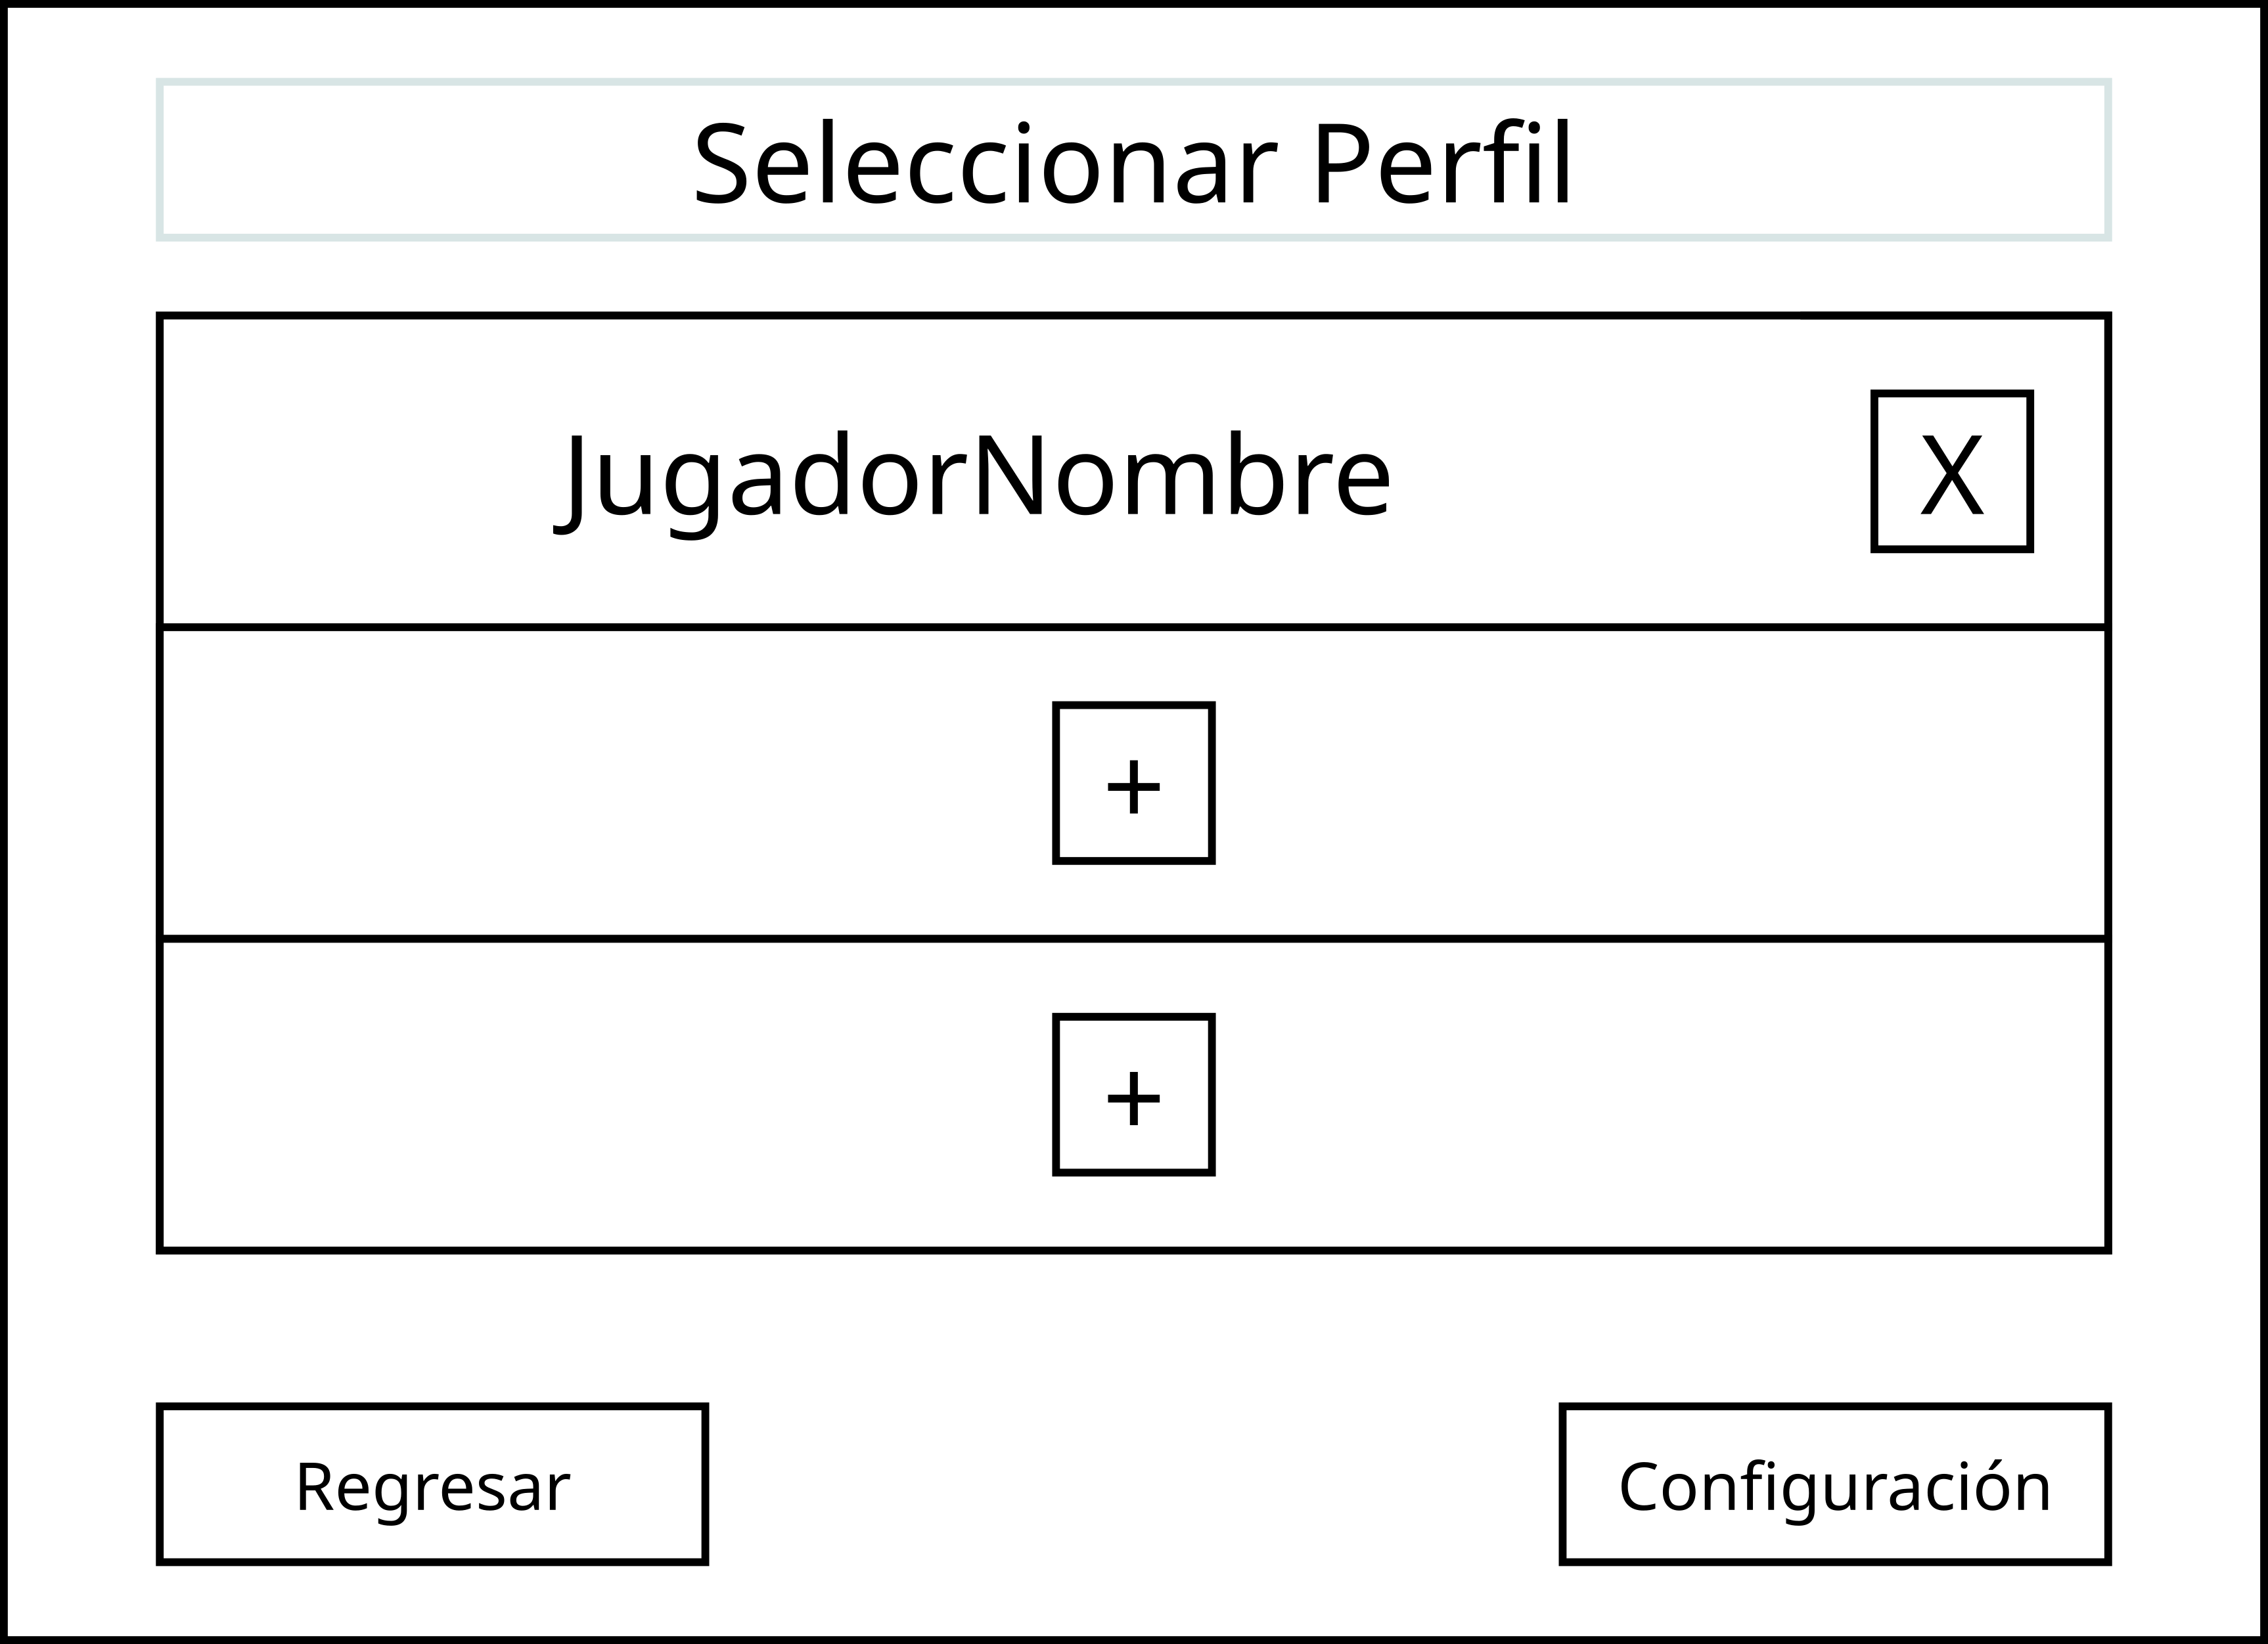
\includegraphics[width=0.6\textwidth]{5-Cuerpo/Chapter5/I3.png} %
    \caption{Interfaz de visualización de perfil}
    \label{fig:Interface_Perfil}
\end{figure}
\begin{enumerate}\setcounter{enumi}{10}
    \item 11
    \item 12
    \item 13
\end{enumerate}

\subsubsection{Modo configuración de partida}
\begin{figure}[H]
    \centering
    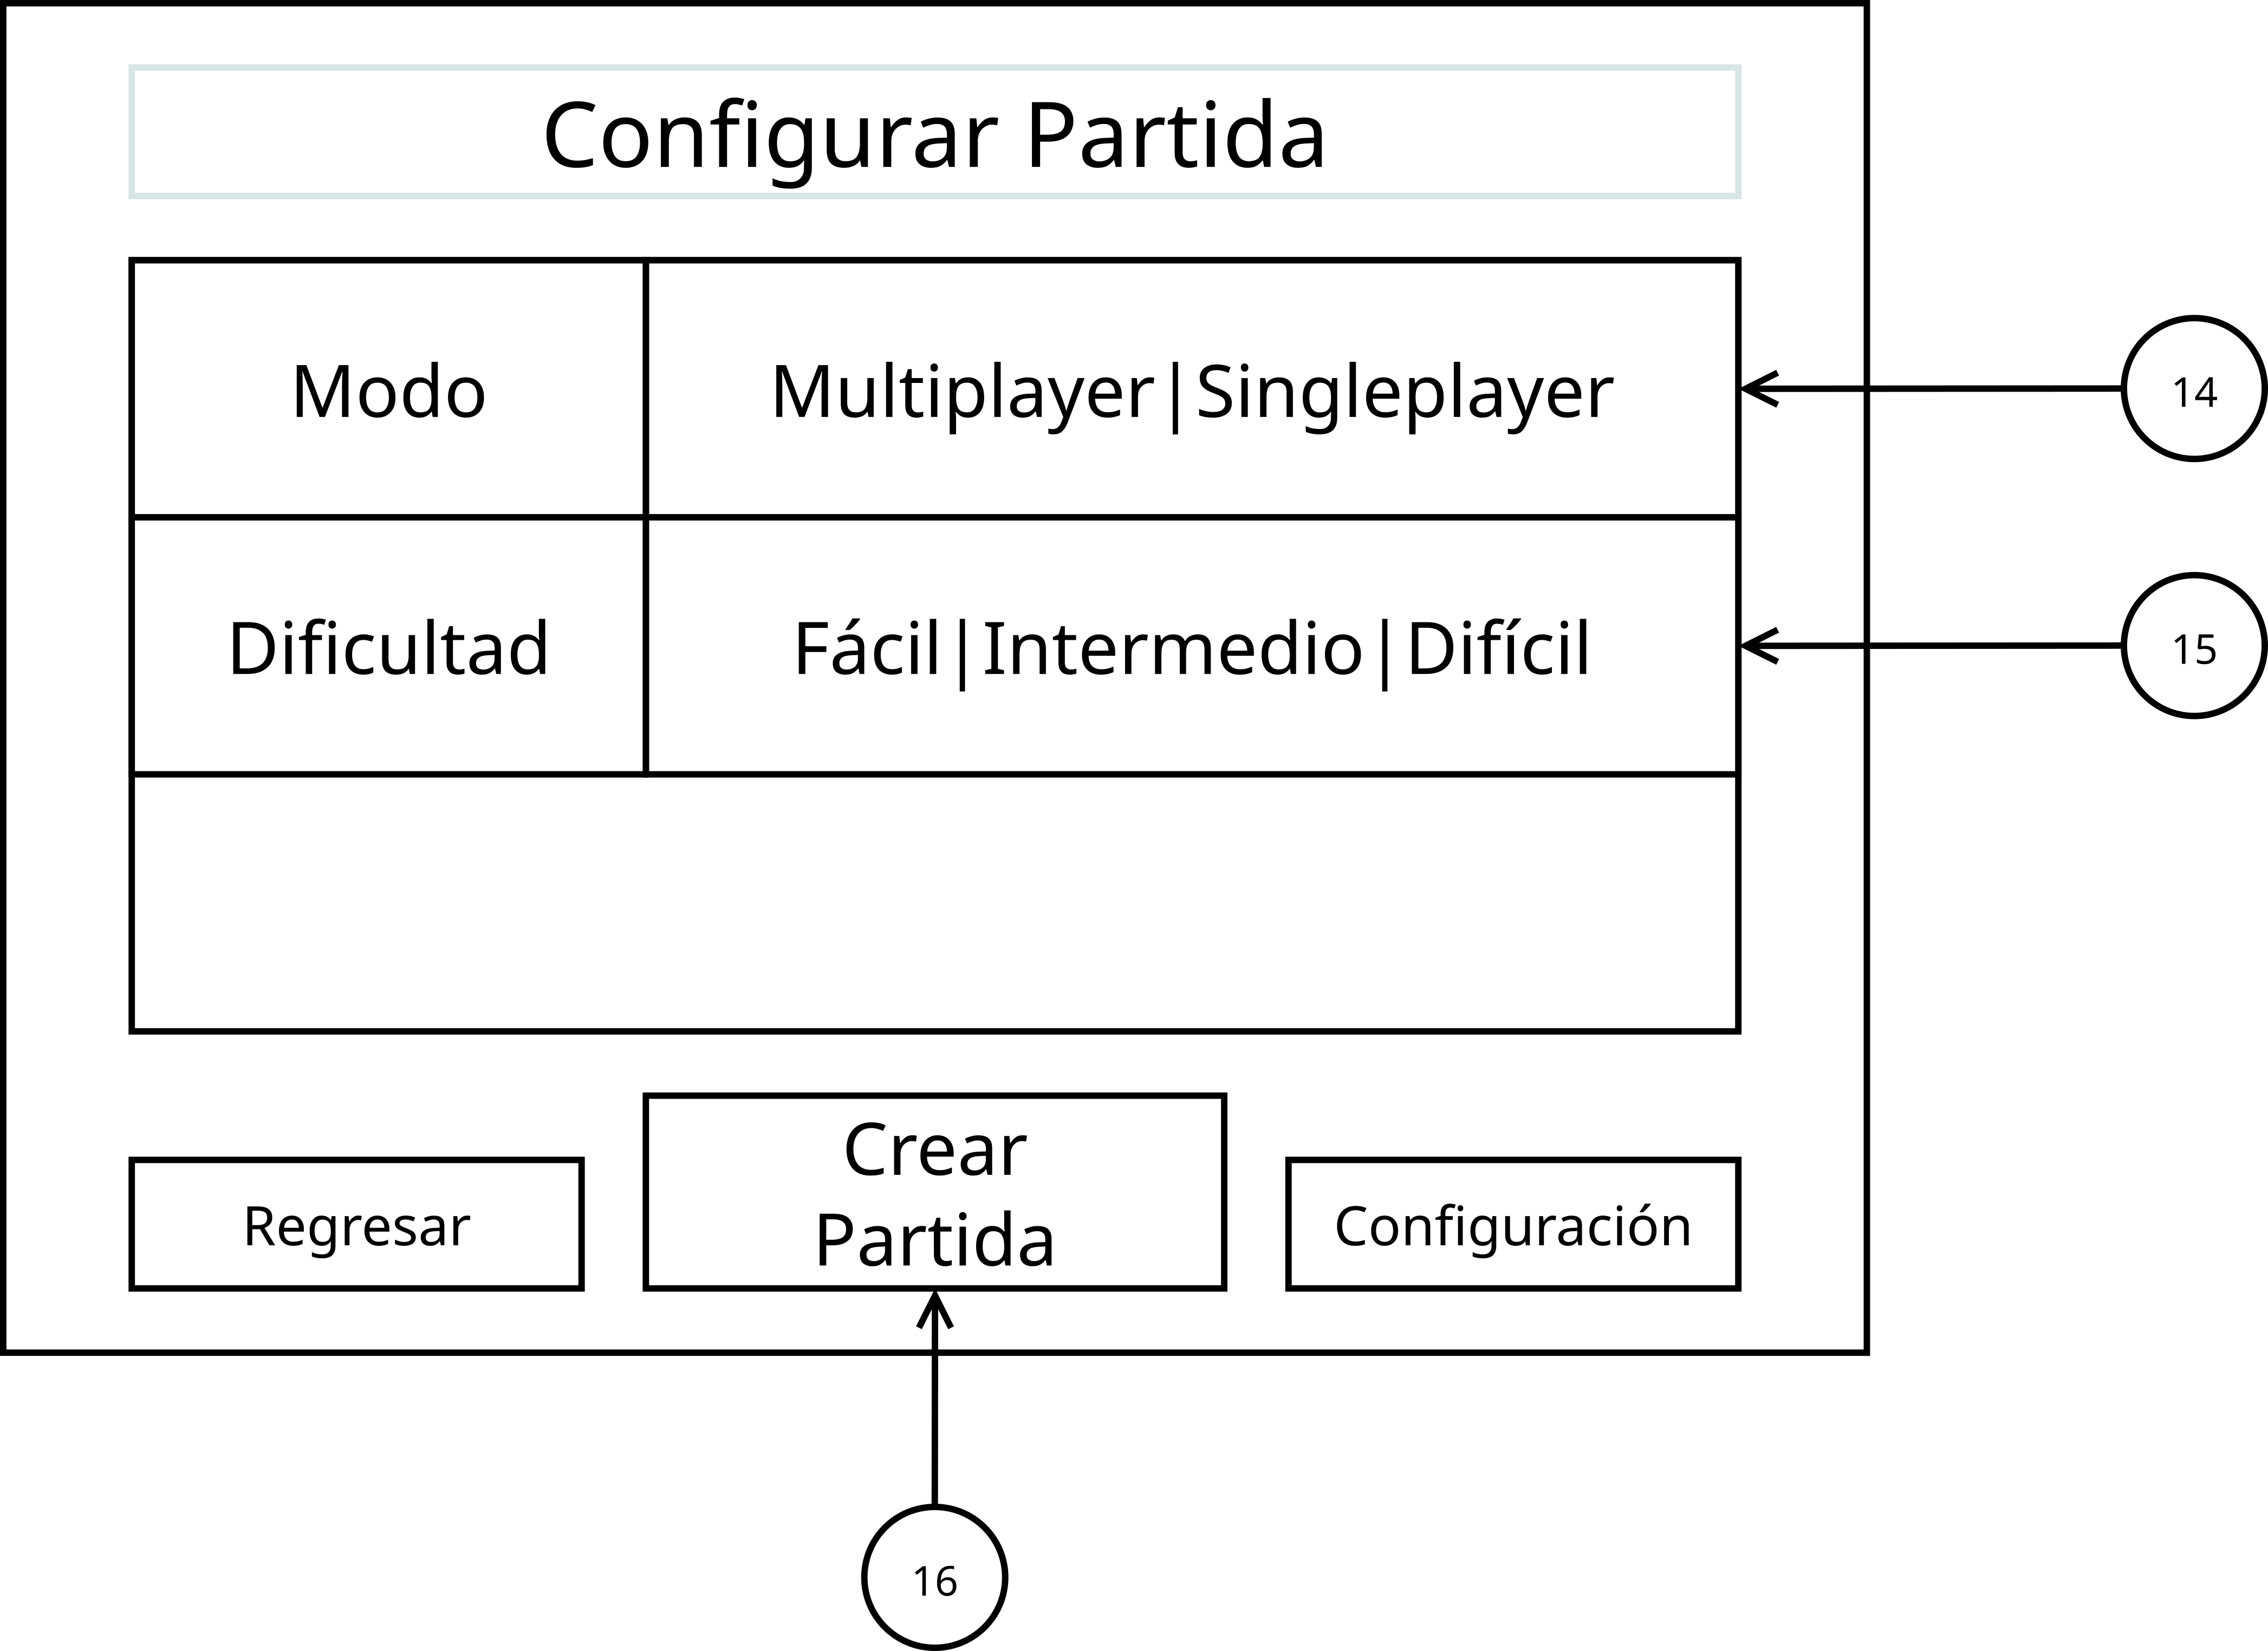
\includegraphics[width=0.6\textwidth]{5-Cuerpo/Chapter5/I4.png} %
    \caption{Interfaz del menú de configuración de partida}
    \label{fig:Interface_Configuracion_Partida}
\end{figure}
\begin{enumerate}\setcounter{enumi}{13}
    \item 14
    \item 15
    \item 16
\end{enumerate}

\subsubsection{Modo selección de personaje}
\begin{figure}[H]
    \centering
    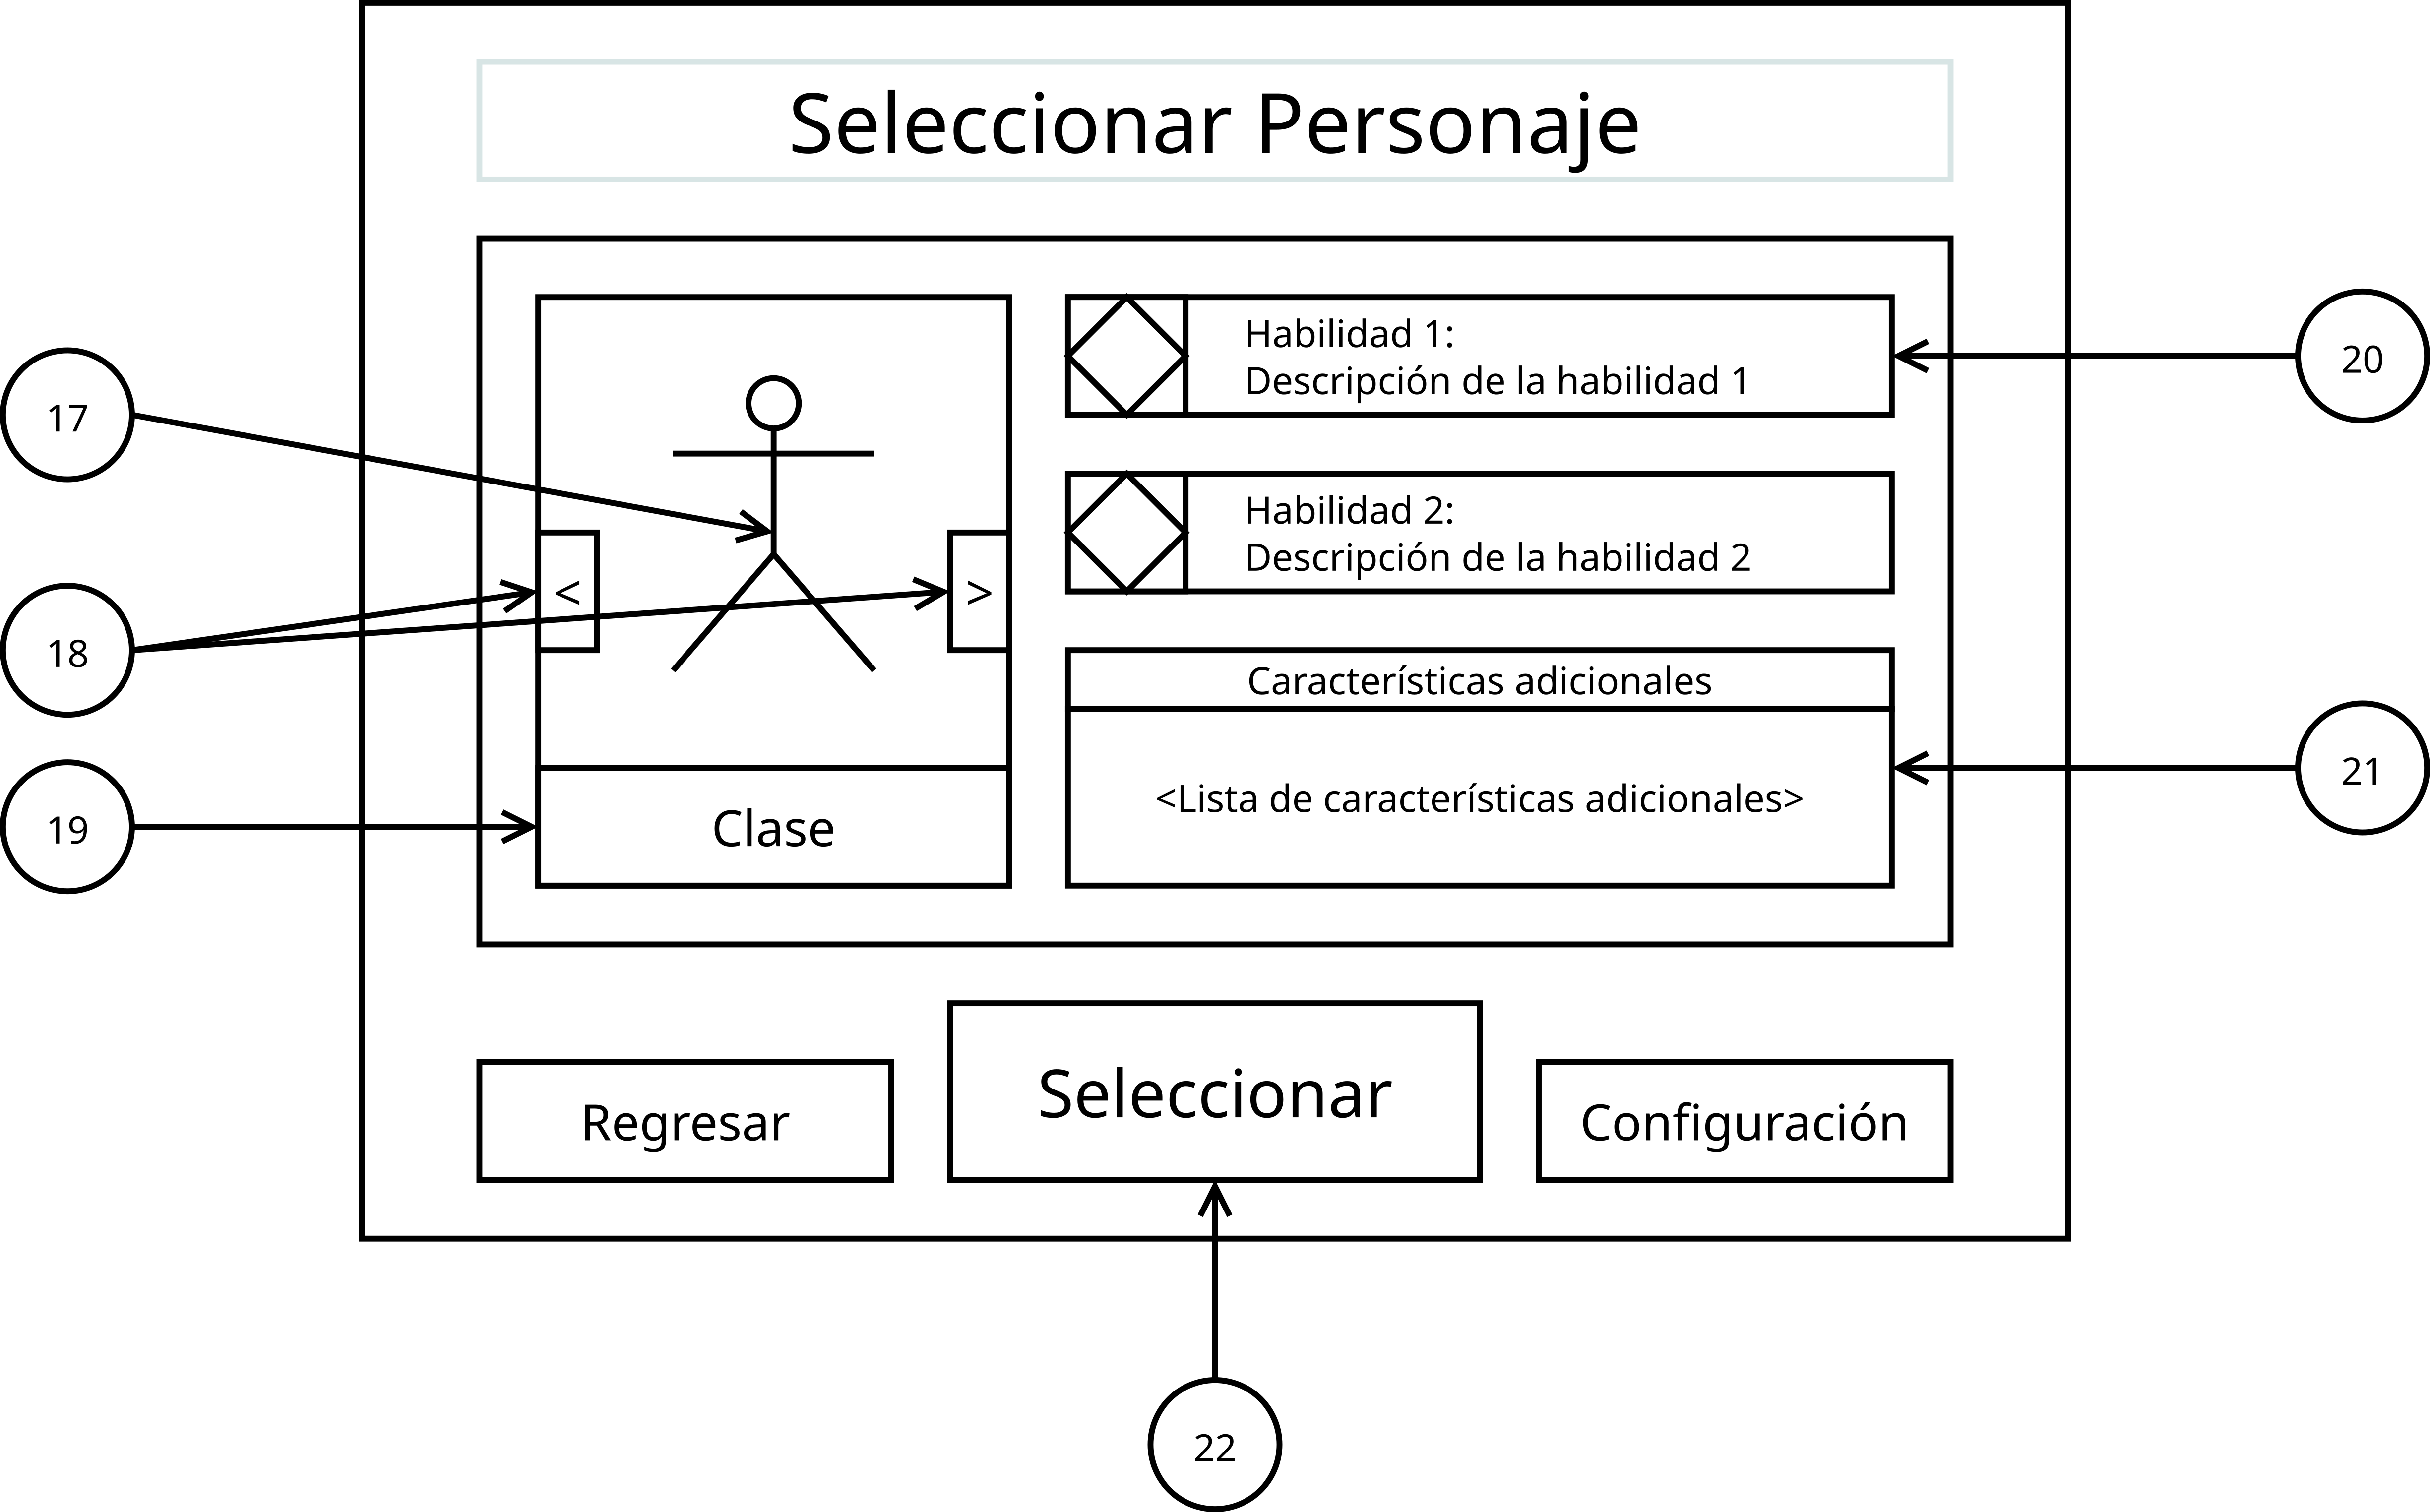
\includegraphics[width=0.6\textwidth]{5-Cuerpo/Chapter5/I5.png} %
    \caption{Interfaz del menú de selección de personaje}
    \label{fig:Interface_Seleccion_Personaje}
\end{figure}
\begin{enumerate}\setcounter{enumi}{16}
    \item 17
    \item 18
    \item 19
    \item 20
    \item 21
    \item 22
\end{enumerate}

\subsubsection{Modo partida}
\begin{figure}[H]
    \centering
    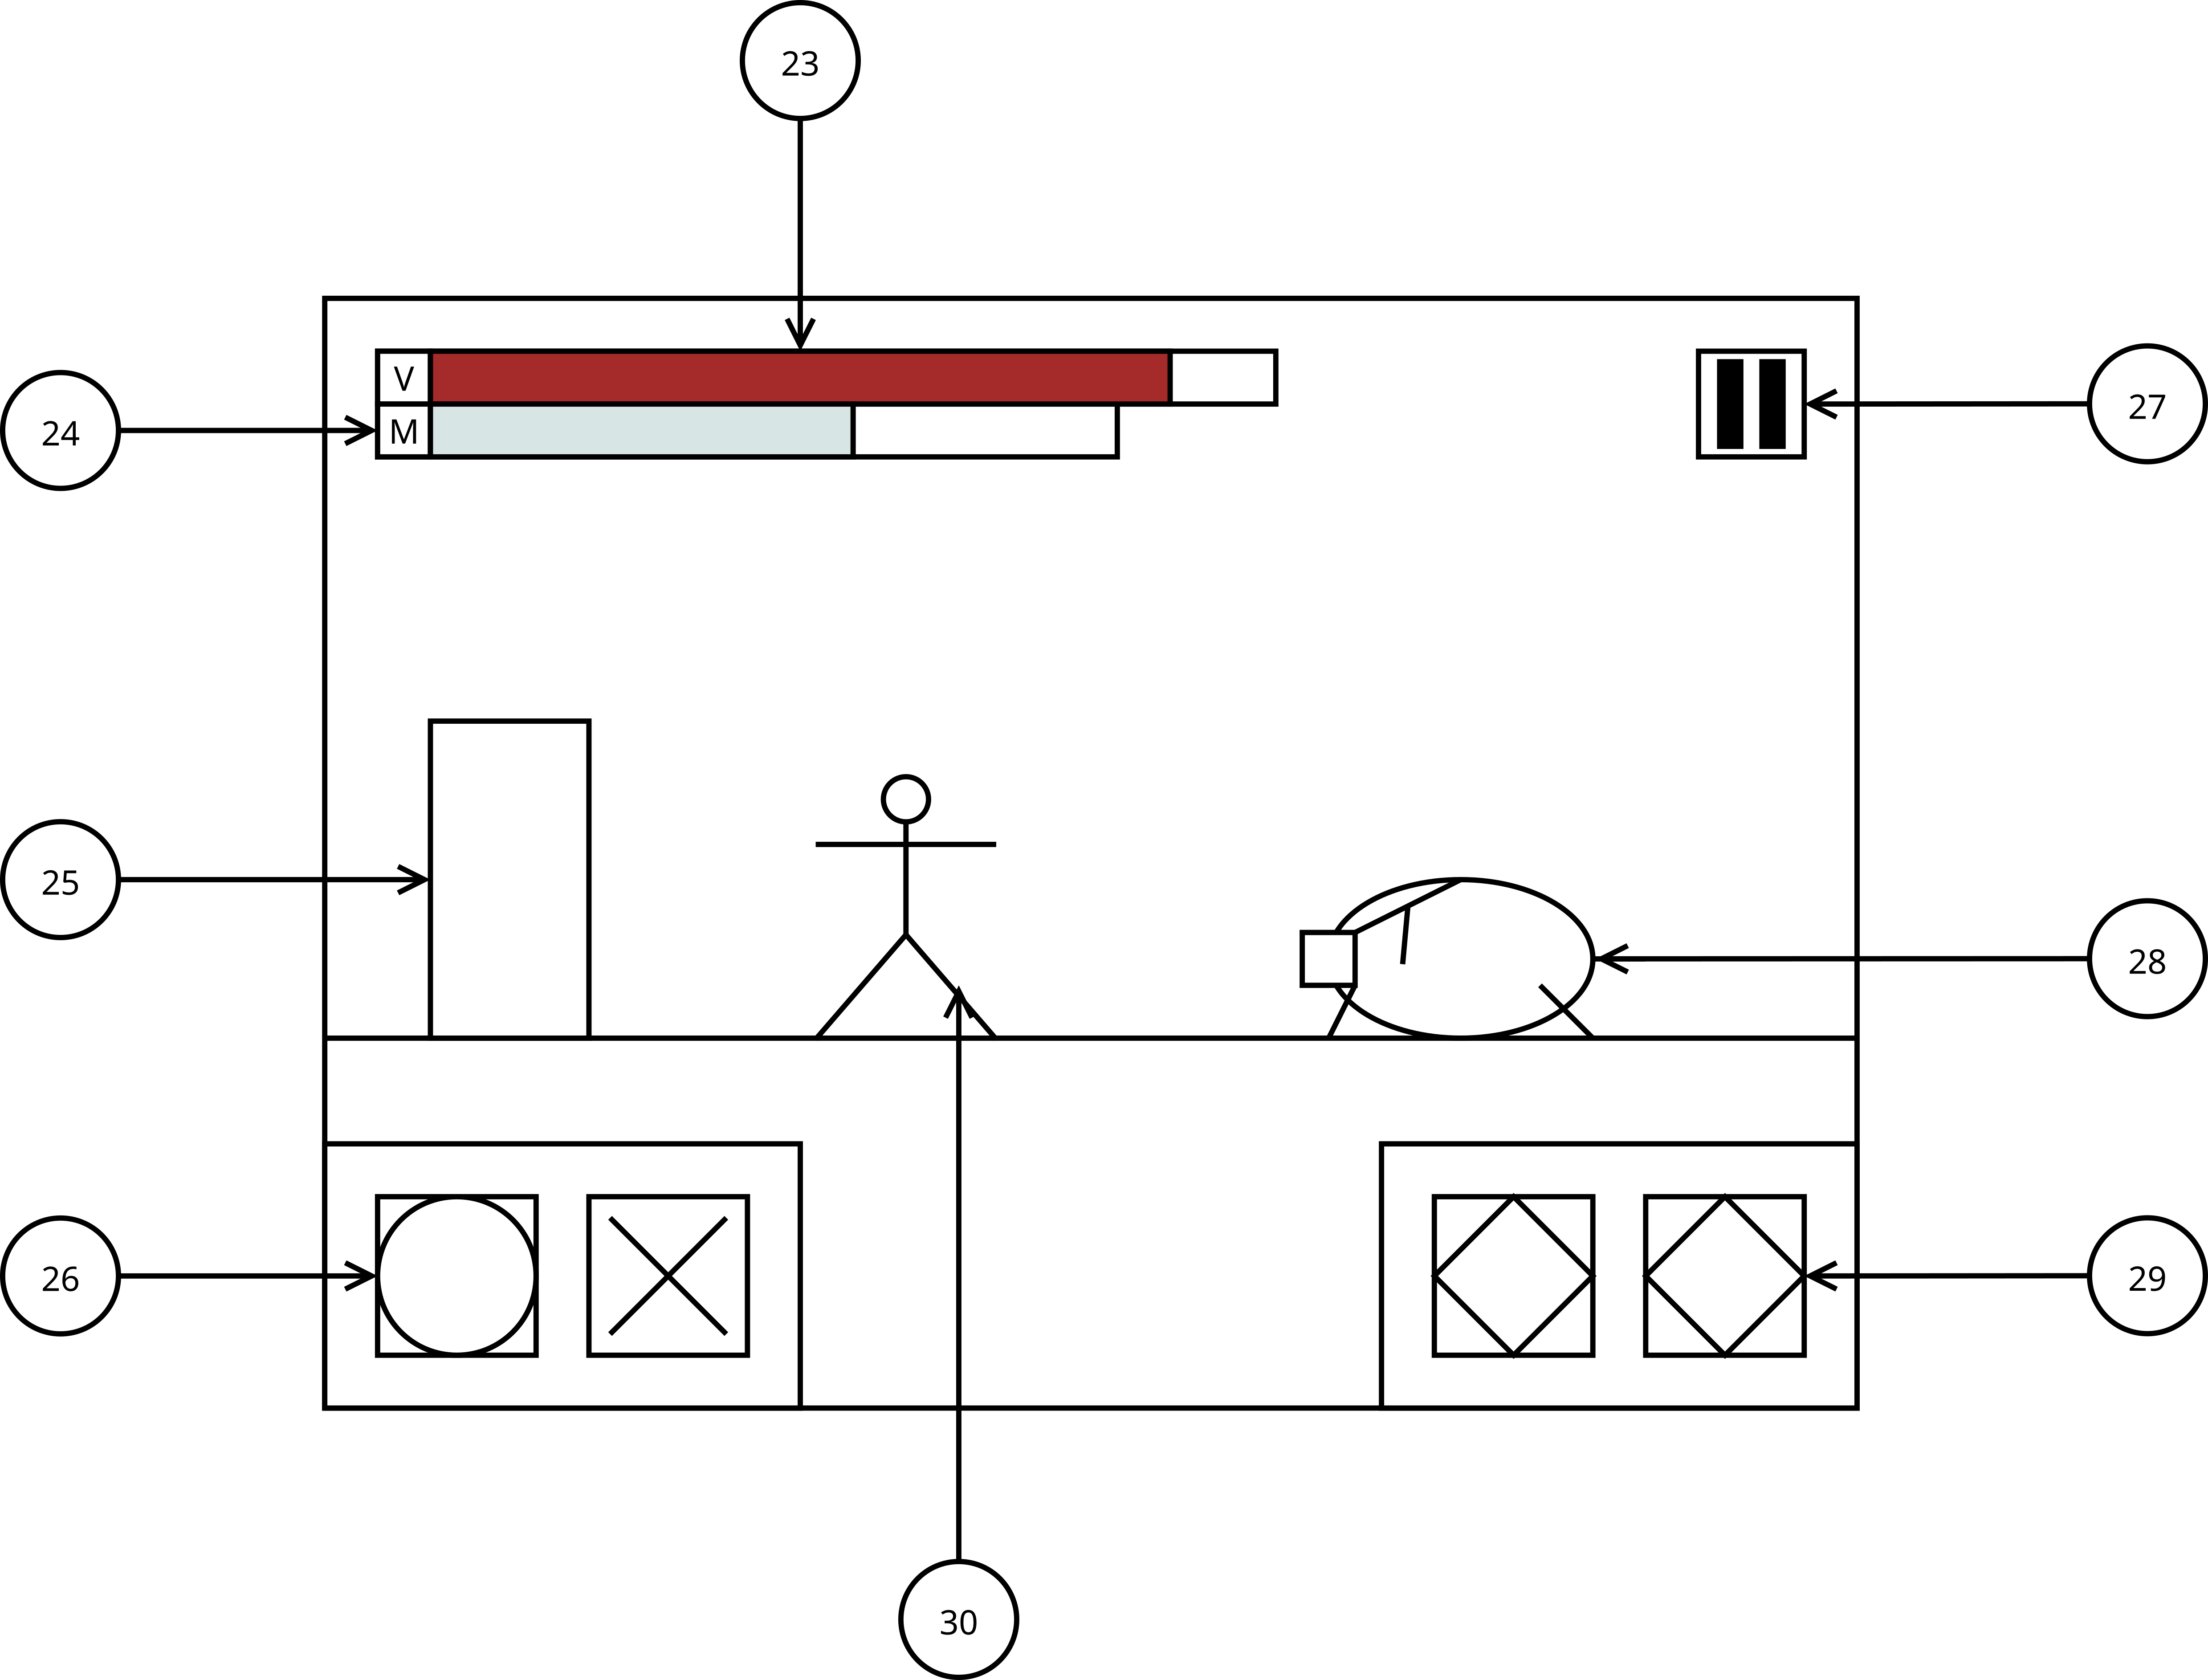
\includegraphics[width=0.6\textwidth]{5-Cuerpo/Chapter5/I6.png} %
    \caption{Interfaz de la partida}
    \label{fig:Interface_Partida}
\end{figure}
\begin{enumerate}\setcounter{enumi}{22}
    \item 23
    \item 24
    \item 25
    \item 26
    \item 27
    \item 28
    \item 29
    \item 30
\end{enumerate}

\subsubsection{Modo pausa}
\begin{figure}[H]
    \centering
    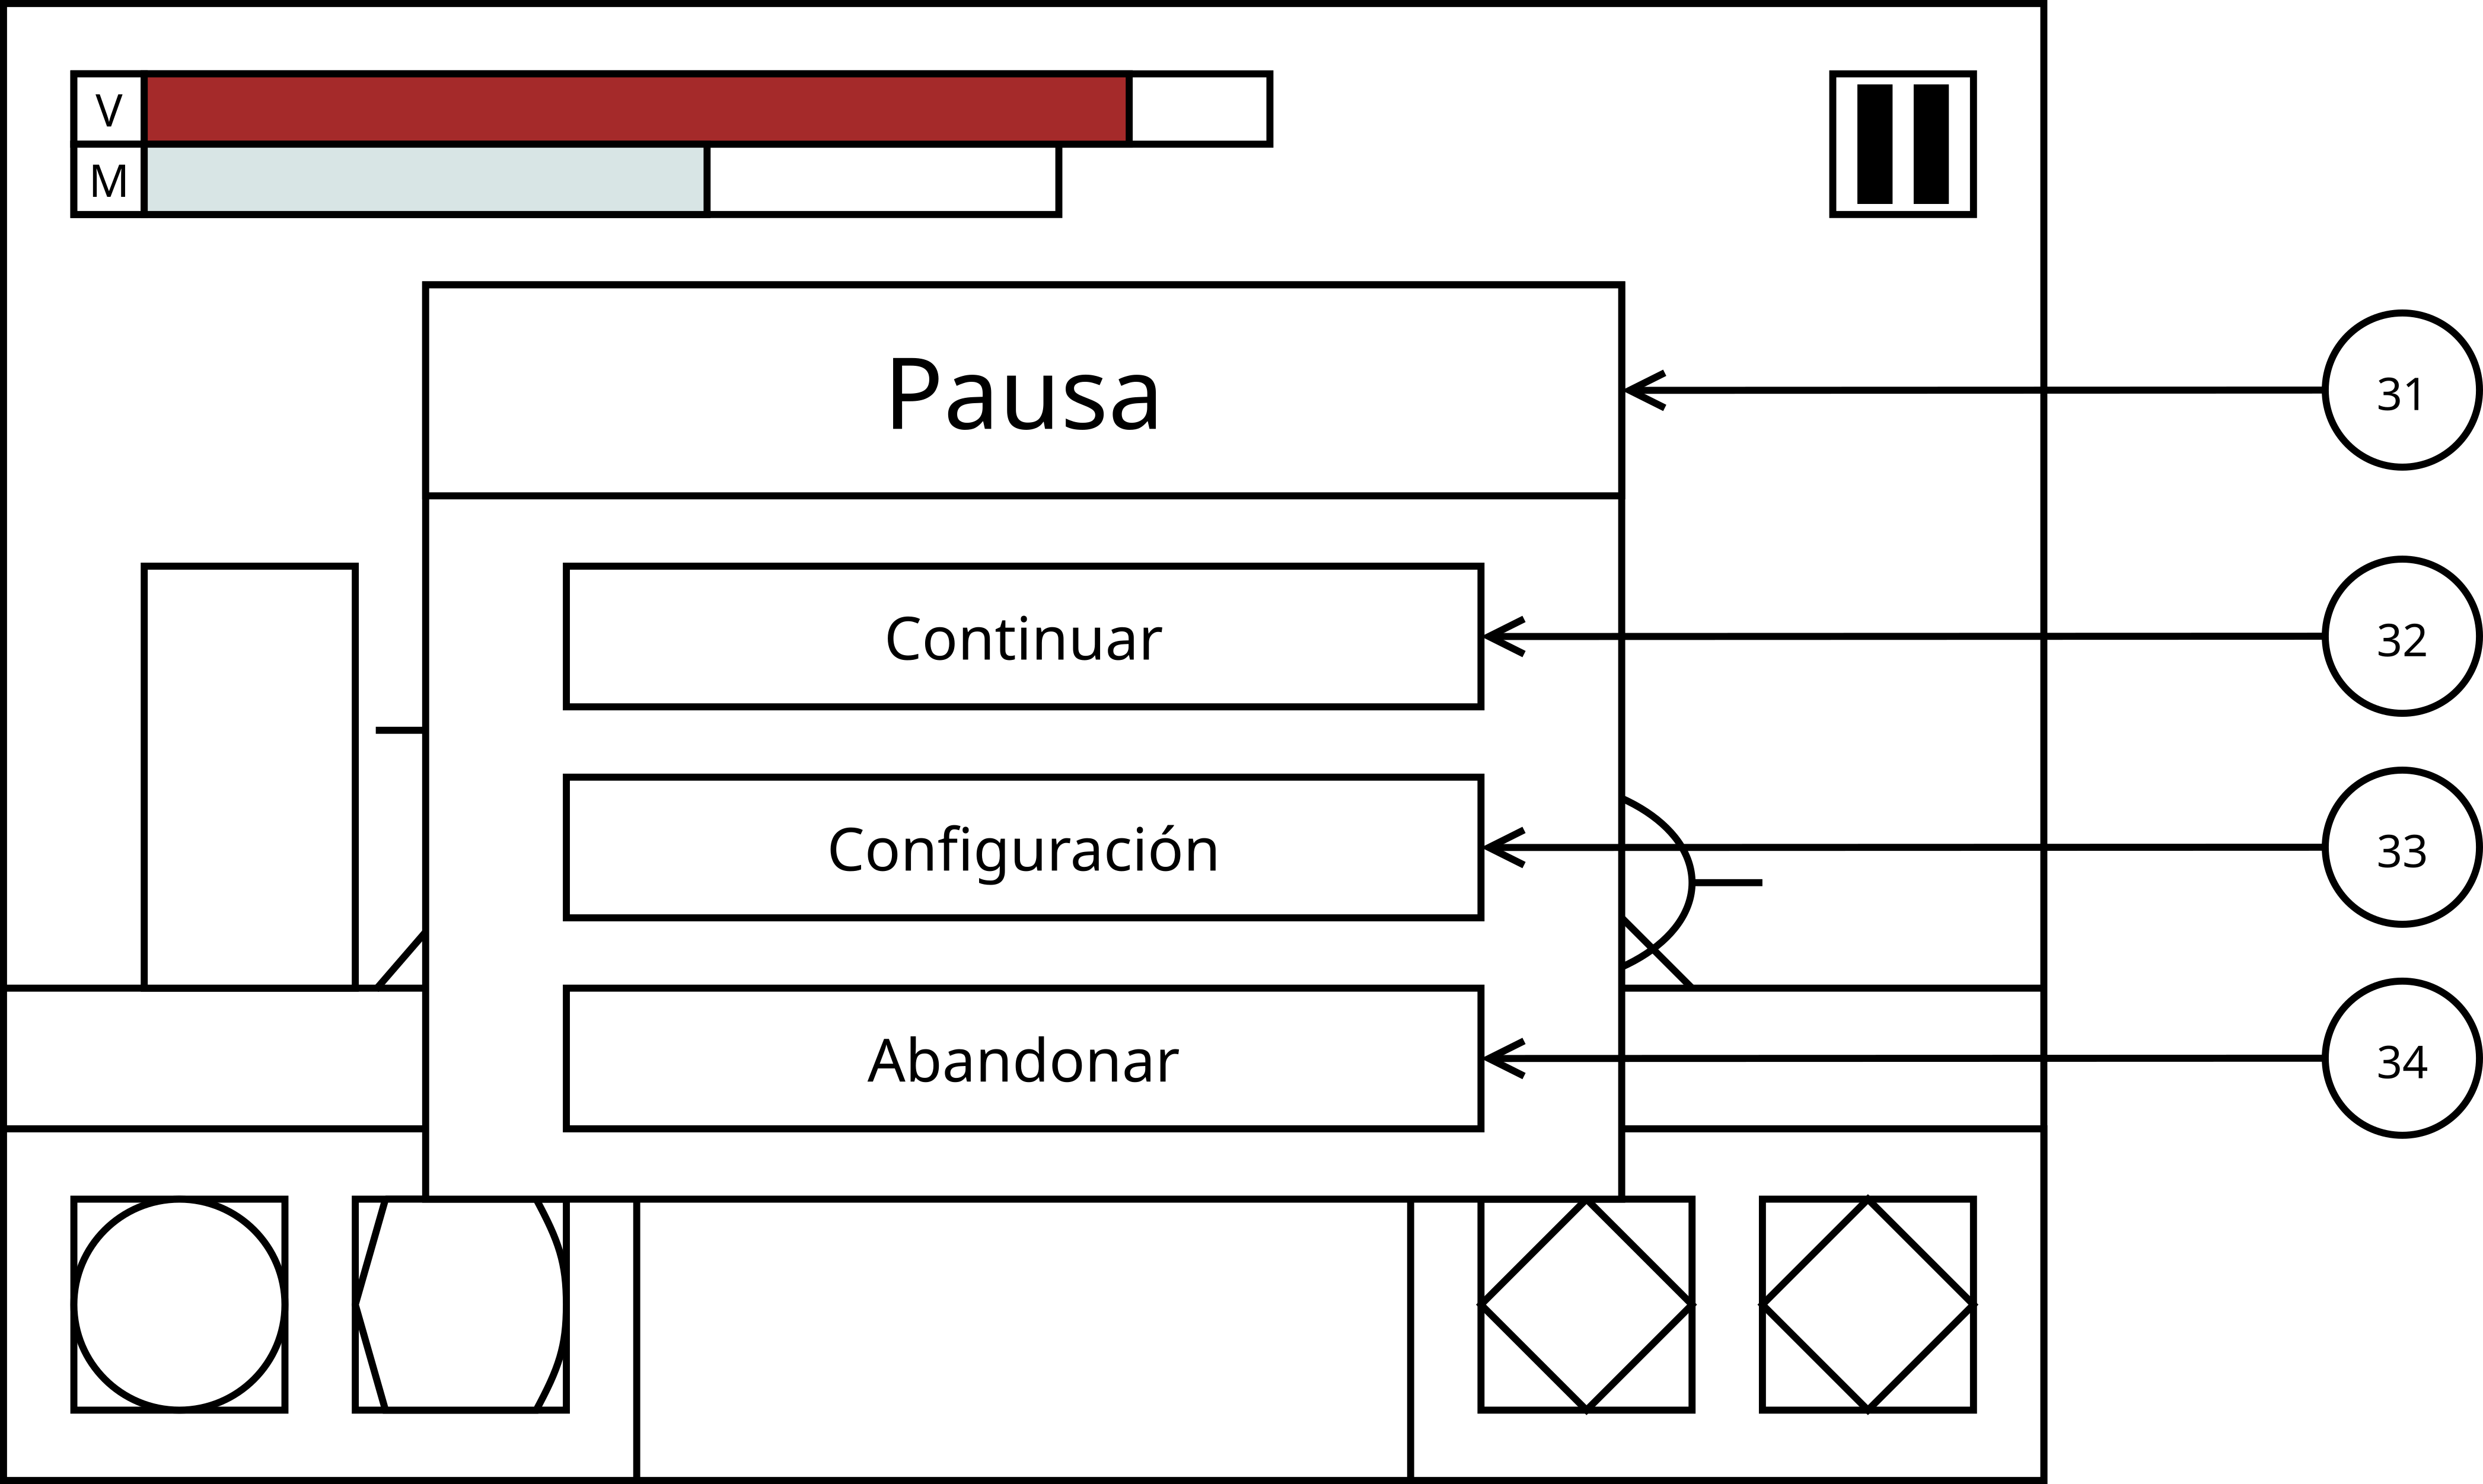
\includegraphics[width=0.6\textwidth]{5-Cuerpo/Chapter5/I7.png} %
    \caption{Interfaz del menú de pausa}
    \label{fig:Interface_Pausa}
\end{figure}
\begin{enumerate}\setcounter{enumi}{30}
    \item 31
    \item 32
    \item 33
    \item 34
\end{enumerate}

\subsubsection{Modo victoria}
\begin{figure}[H]
    \centering
    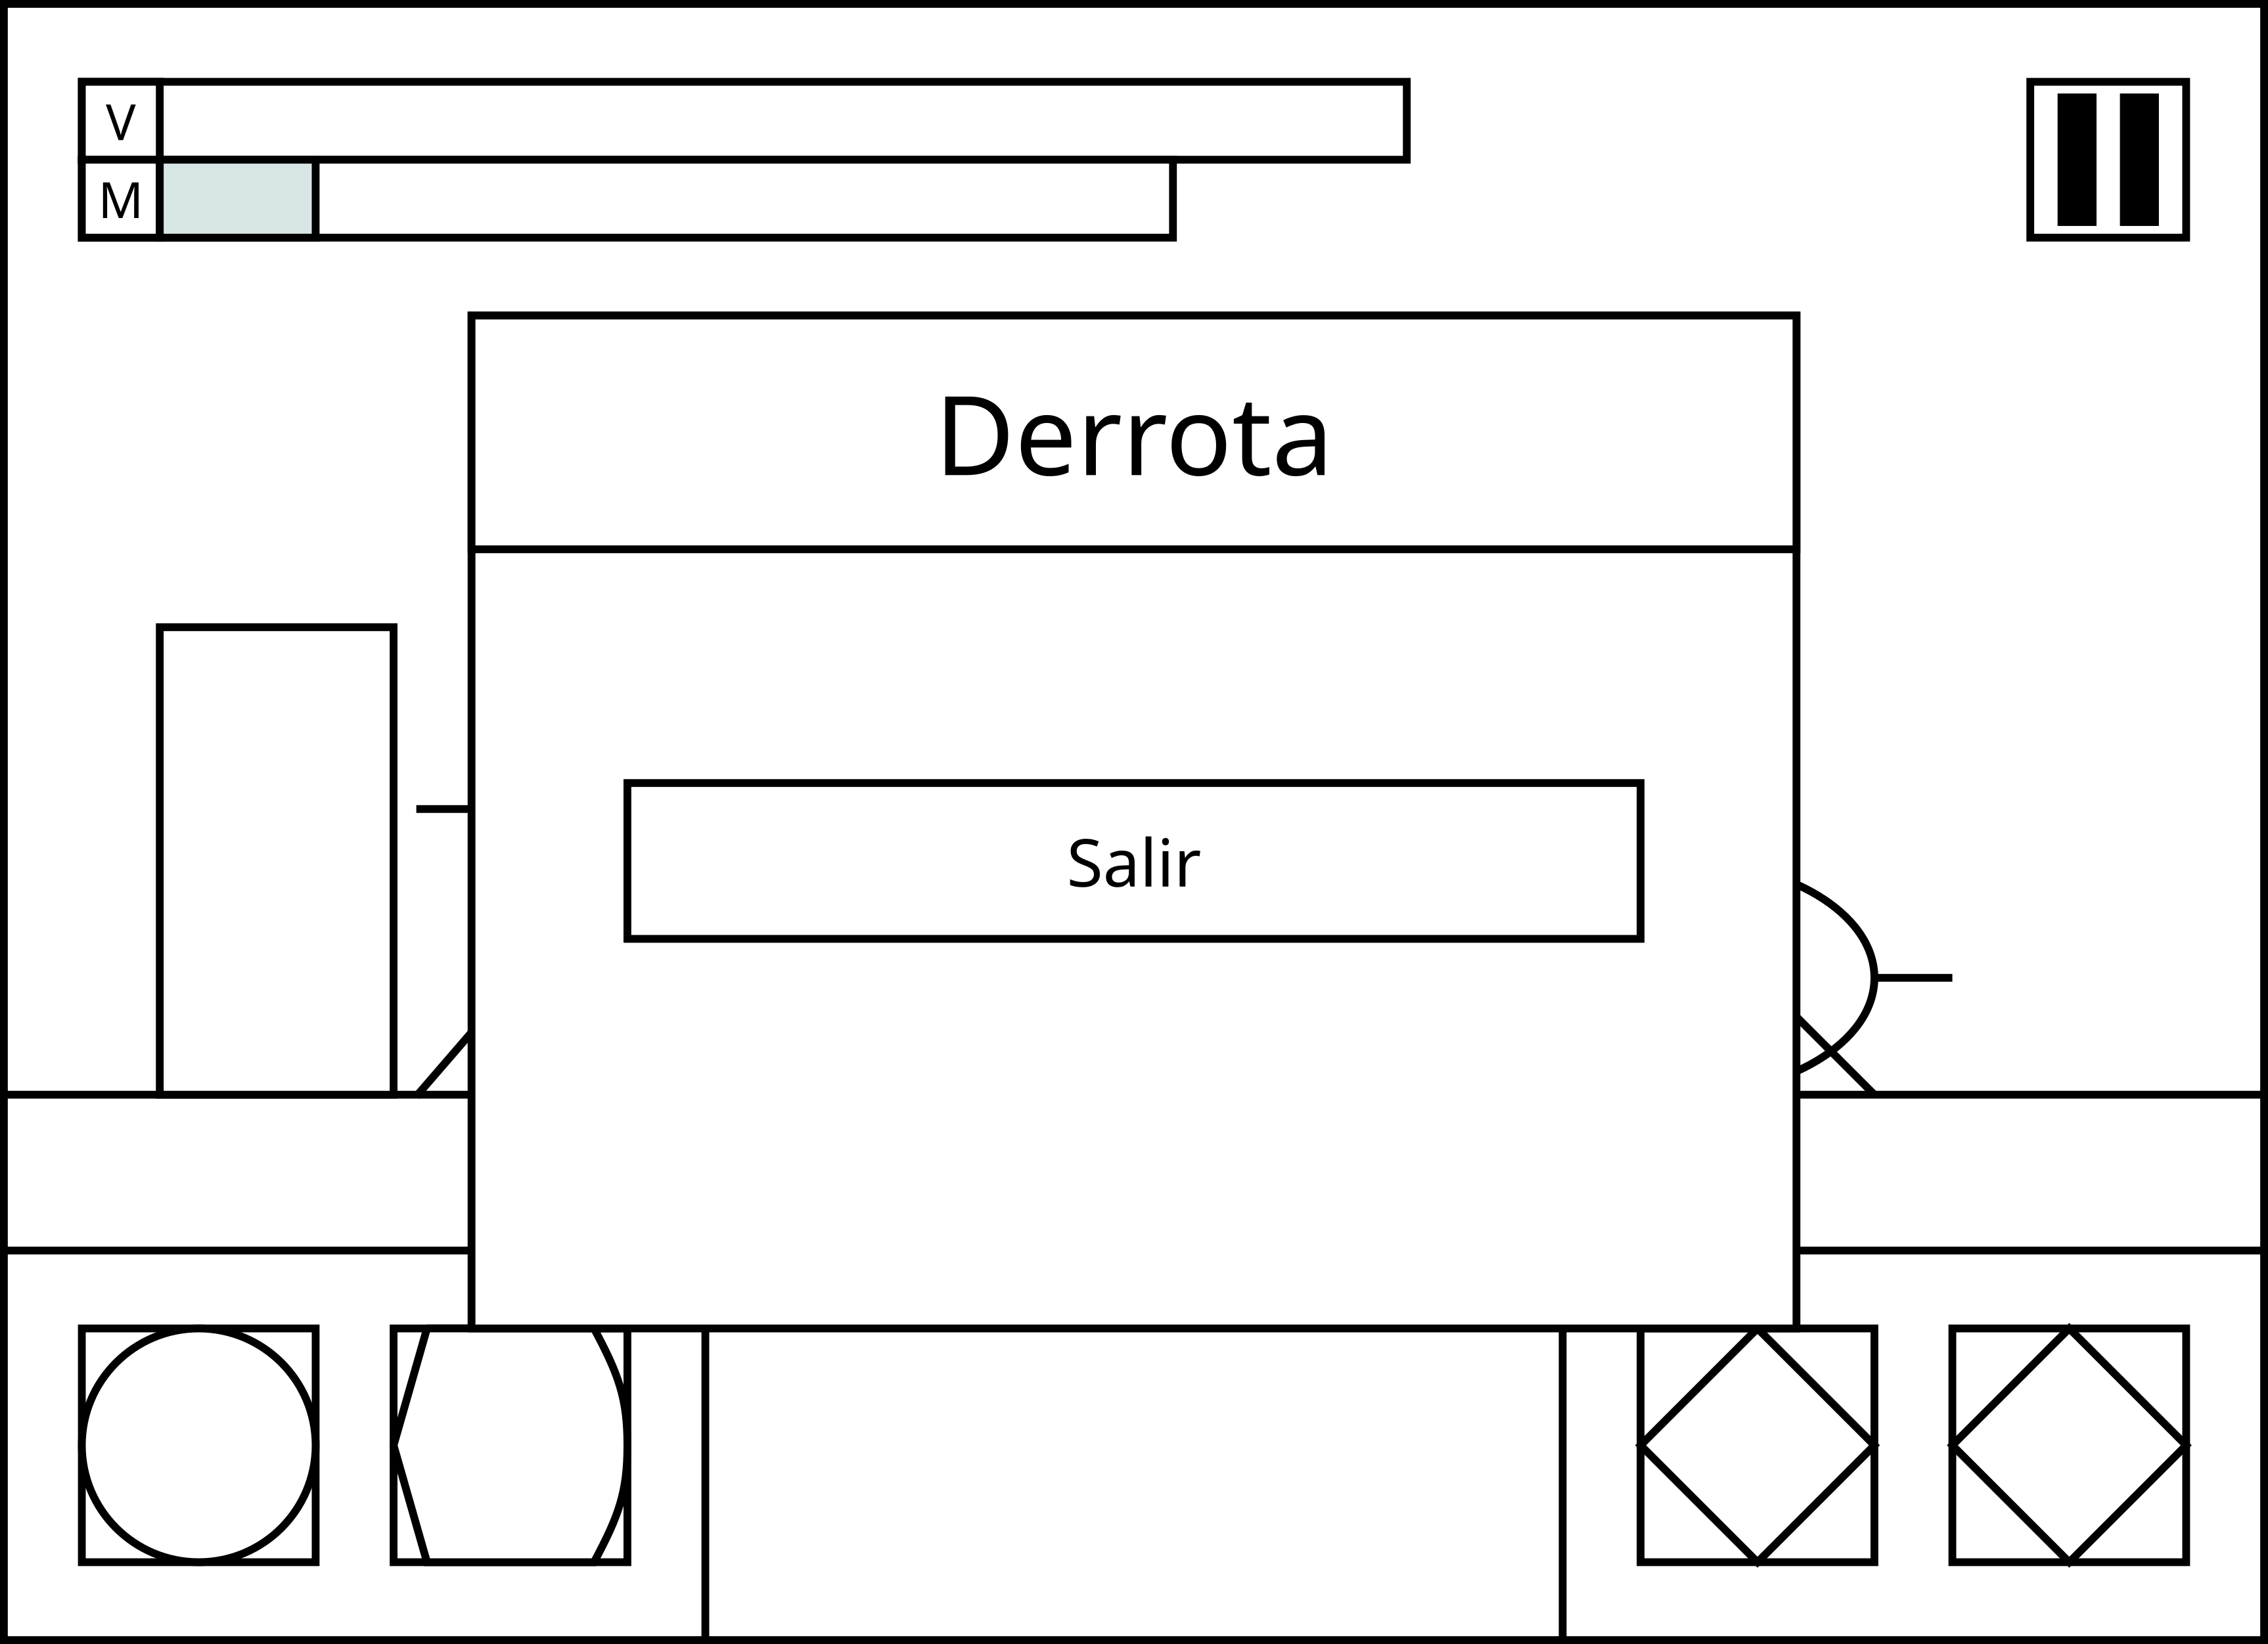
\includegraphics[width=0.6\textwidth]{5-Cuerpo/Chapter5/I8.png} %
    \caption{Interfaz del menú de victoria}
    \label{fig:Interface_Victoria}
\end{figure}
\begin{enumerate}\setcounter{enumi}{34}
    \item 35
\end{enumerate}

\subsubsection{Modo derrota}
\begin{figure}[H]
    \centering
    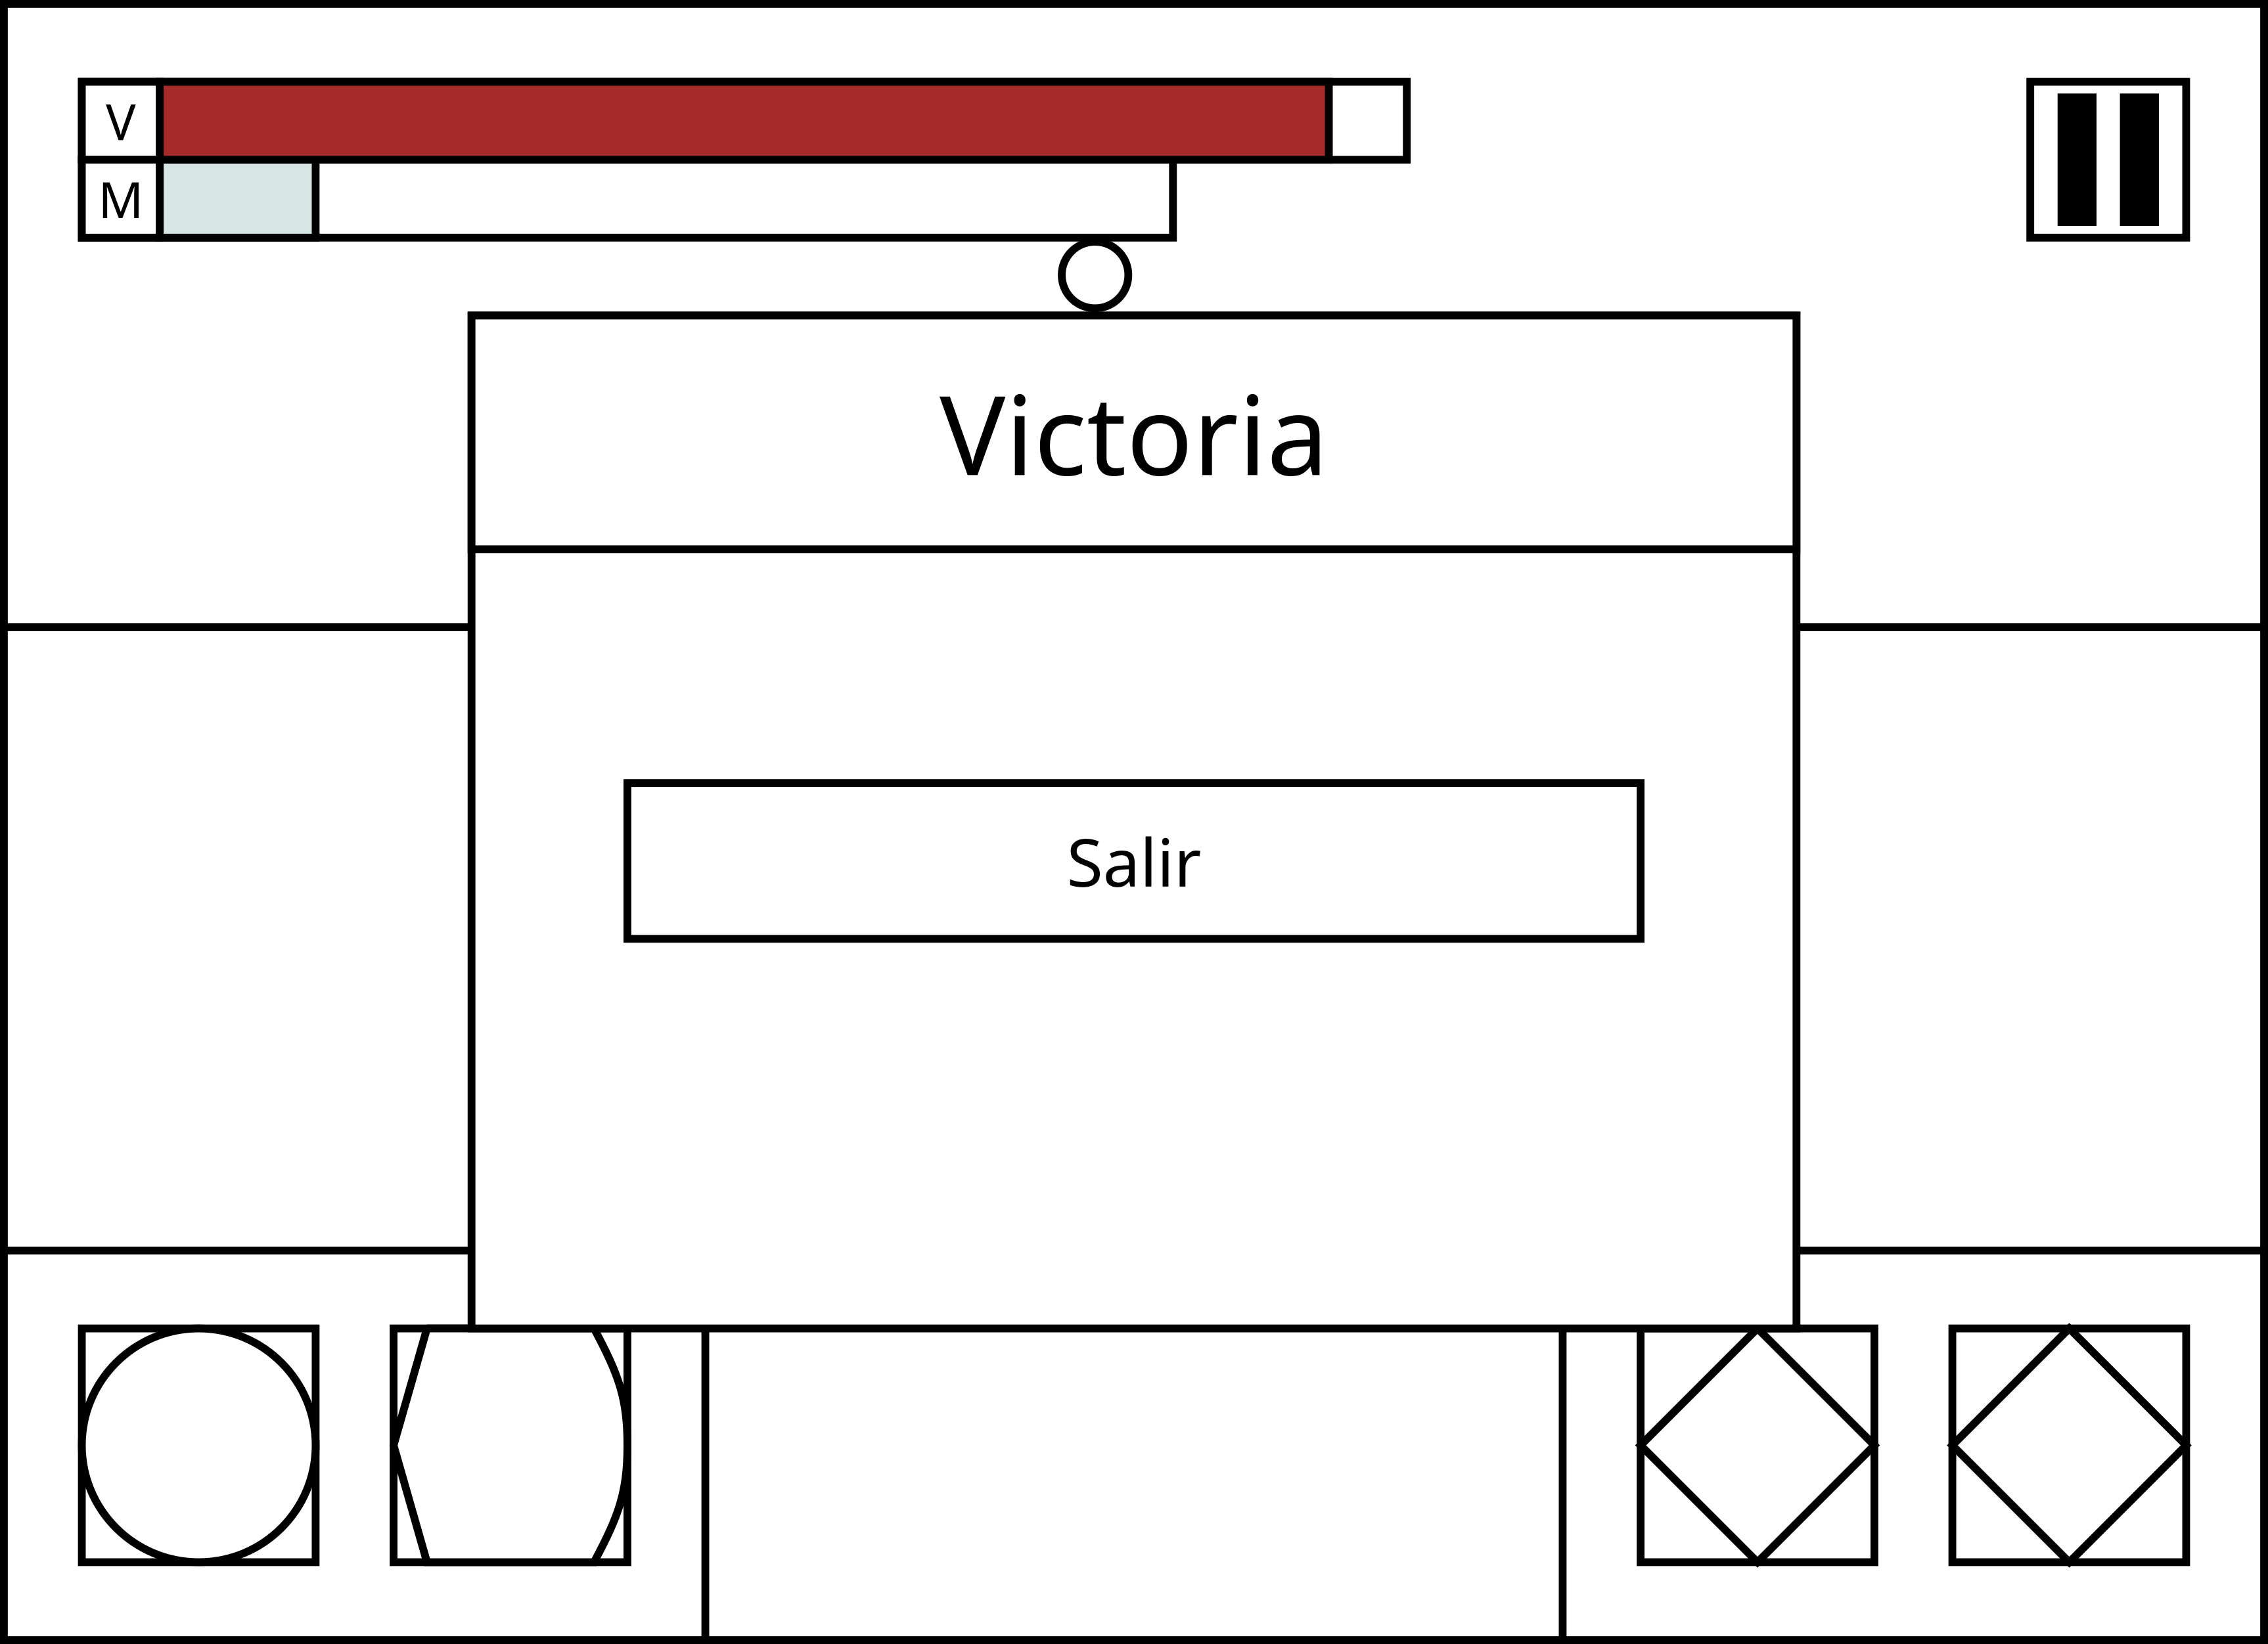
\includegraphics[width=0.4\textwidth]{5-Cuerpo/Chapter5/I9.png} %
    \caption{Interfaz del menú de derrota}
    \label{fig:Interface_Derrota}
\end{figure}


\subsubsection{Modo configuración general}
\begin{figure}[H]
    \centering
    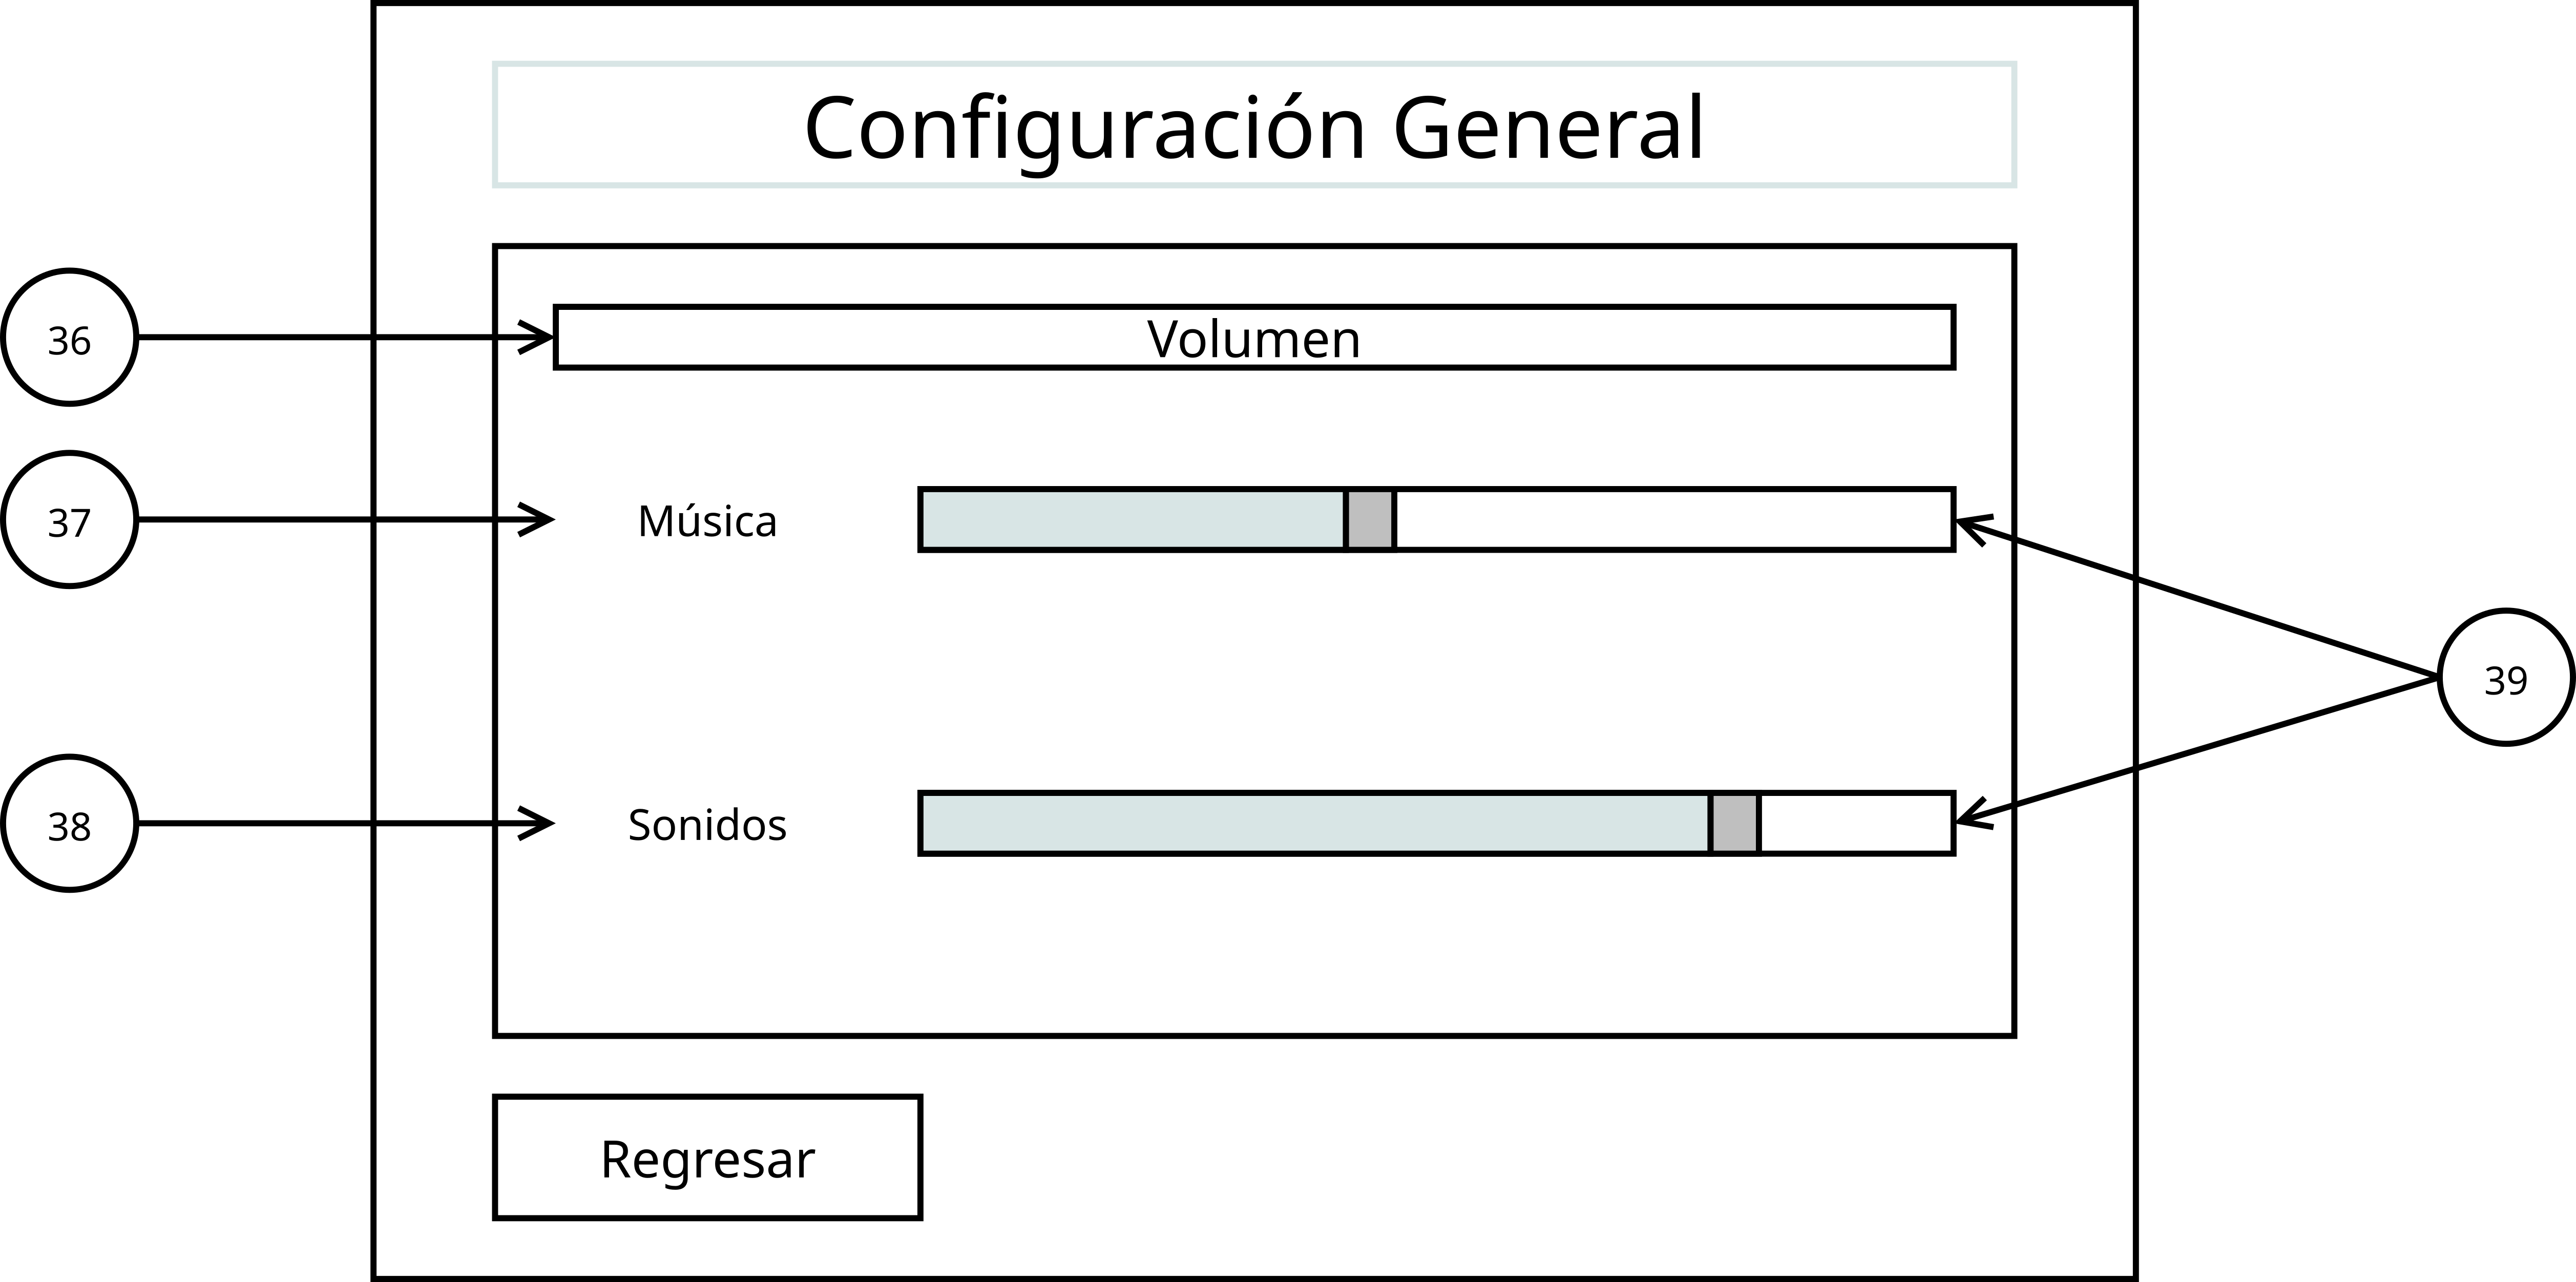
\includegraphics[width=0.6\textwidth]{5-Cuerpo/Chapter5/I10.png} %
    \caption{Interfaz del menú de configuración general}
    \label{fig:Interface_Configuracion_General}
\end{figure}
\begin{enumerate}\setcounter{enumi}{35}
    \item 36
    \item 37
    \item 38
    \item 39
\end{enumerate}